\documentclass[a4paper, notitlepage, 9pt]{extreport}
\usepackage[italian]{babel}
\usepackage[T1]{fontenc}
\usepackage[utf8]{inputenc}
\usepackage{amsmath}
\usepackage{amsfonts}
\usepackage{amsthm}
\usepackage{frontespizio}
\usepackage{hyperref}
\hypersetup{hidelinks,
	colorlinks = true,
	urlcolor = black, 
	linkcolor = black}
\usepackage[margin=3cm]{geometry}
\usepackage{booktabs}
\usepackage{fancyhdr}
\usepackage{listings}
\setcounter{tocdepth}{4}
\usepackage{stmaryrd}
\usepackage[strict]{changepage}
\usepackage{libertine}
\usepackage{textcomp}
\usepackage{float}
\usepackage{multicol}
\usepackage{makecell}
\usepackage{stmaryrd}
\usepackage{amssymb}
\usepackage{caption}
\renewcommand\theadalign{bc}
\renewcommand\theadfont{\bfseries}
\renewcommand\theadgape{\Gape[4pt]}
\renewcommand\cellgape{\Gape[4pt]}

\lstset{basicstyle=\ttfamily\small}

\makeatletter
\newcommand*{\toccontents}{\@starttoc{toc}}
\makeatother

\begin{document}
	\title{\textbf{\underline{Verifica Automatica di Sistemi}}}
	\date{Giugno 2018}
	\author{Colognese, Rossini}
	\maketitle
	
	\toccontents

\chapter*{Transition System}
\addcontentsline{toc}{chapter}{Transition System}
Dato un sistema reale, esegue un'astrazione modellandone: gli stati, le transizioni tra essi e informazioni aggiuntive (comunicazione e proprietà degli stati).\\\\
Il \textit{\textbf{Transition System} (TS)} è una tupla: $\mathcal{T} = (S, Act, \longrightarrow, S_0, AP, L)$, dove:
\begin{itemize}
	\item $S$ è l'insieme degli stati (con $S_0 \in S$);
	\item $Act$ è l'insieme delle azioni;
	\item $\longrightarrow ~\subseteq S \times Act \times S$ è la relazione di transizione;
	\item $AP$ è l'insieme delle proposizioni atomiche;
	\item $L: S \rightarrow 2^{AP}$ la funzione di etichettamento.
\end{itemize}
\textit{Esecuzioni}: sequenze massimali di transizioni. $s_0 \rightarrow^{a_1} s_1 \rightarrow^{a_2} s_3 \rightarrow^{a_3} \dots$\\
\textit{Effect-function}: $Act \times Eval(Var) \rightarrow Eval(Var)$\\
\textit{\textbf{Reach}}$(\mathcal{T}) = $ insieme di tutti gli stati raggiungibili da uno stato inziale attraverso qualche esecuzione.
\begin{multicols}{2}
	\begin{figure}[H]
		\centering
		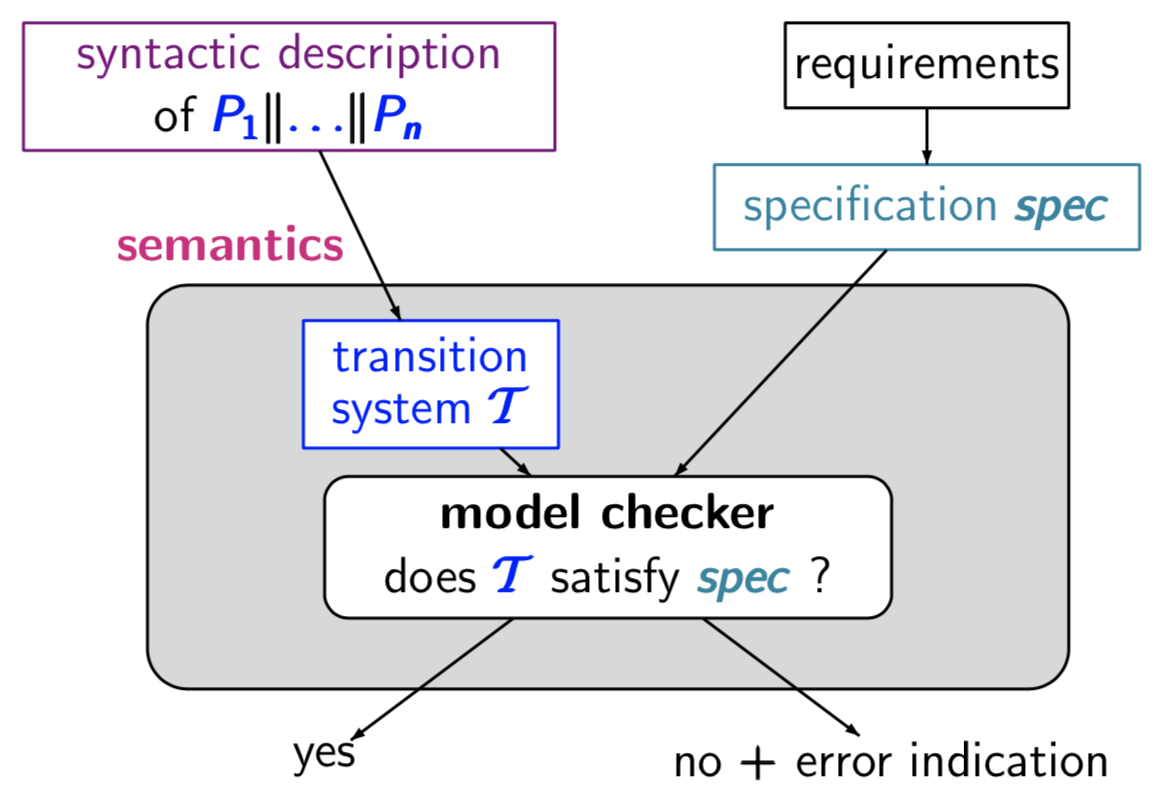
\includegraphics[scale=0.23]{MC}
	\end{figure}
	\columnbreak
	\begin{figure}[H]
		\centering
		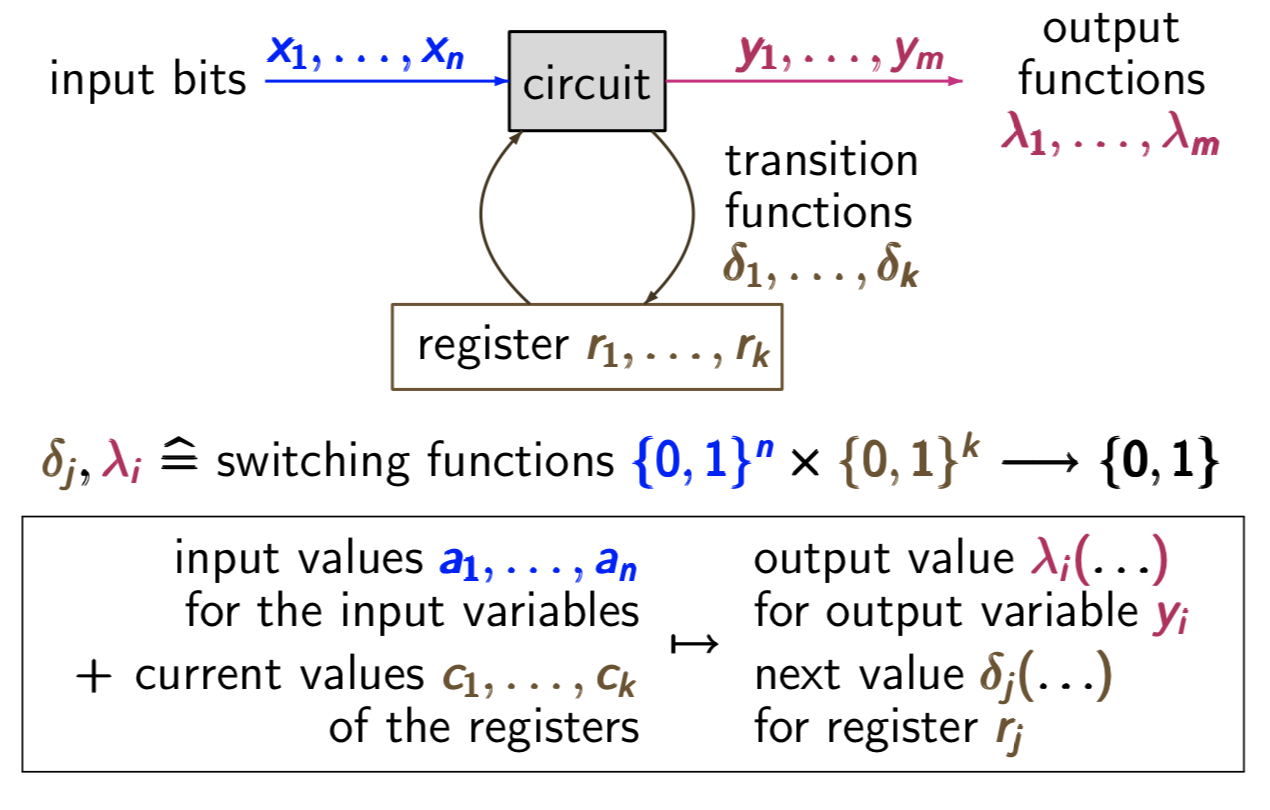
\includegraphics[scale=0.25]{MC2}
	\end{figure}
\end{multicols}



\section*{Program Graph (PG)}
\addcontentsline{toc}{section}{Program Graph (PG)}
Un \textit{Program Graph} su un'insieme di variabili tipate (\textit{Var}) è una tupla: $\mathcal{P} = (Loc, Act,$ \textit{Effect}$, \hookrightarrow, Loc_0, g_0)$, dove:
\begin{itemize}
	\item $Loc$ è l'insieme delle locazioni (con $L_0 \in L$);
	\item $Act$ è l'insieme delle azioni;
	\item \textit{Effect}: $Act \times Eval(Var) \rightarrow Eval(Var)$;
	\item $\hookrightarrow: Loc \times Cond(Var) \times Act \times Loc$;
	\item $g_0 \in Cond(Var)$: condizione iniziale sulle variabili.
\end{itemize}
Il \textit{TS} corrispondente ad un \textit{PG} ha gli stati della forma: $\langle l, \eta \rangle$, con $l$ locazione corrente e $\eta$ la variabile valutata.
\begin{itemize}
	\item \textit{state space}: $S = Loc \times Eval(Var)$
	\item \textit{initial state}: $S_0 = \{\langle l, \eta \rangle : l \in Loc_0, \eta \vDash g_0 \}$
	\item $\longrightarrow$ è così definita: ~~~if~ $l \hookrightarrow^{g:\alpha} l' \land \eta \vDash g$ ~then~ $\langle l, \eta \rangle \rightarrow^\alpha \langle l',$ \textit{Effect} $(\alpha, \eta) \rangle $
	\item $AP = Loc \cup Cond(Var)$
	\item \textit{labeling function}: $L(\langle l, \eta \rangle) = \{l \} \cup \{g \in Cond(Var): \eta \vDash g \}$
\end{itemize}


\section*{Parallelismo e Comunicazione}
\addcontentsline{toc}{section}{Parallelismo e Comunicazione}
\textit{\textbf{Operatore di Interleaving} (~|||~)}: utilizzato quando le azioni sono indipendenti (non sfruttano le stesse risorse).\\
\textit{Proprietà del diamante}: ~~\textit{\textbf{Effect}}$(\alpha ||| \beta)$ = \textit{\textbf{Effect}}$(\alpha; \beta + \beta; \alpha)$
\begin{multicols}{2}
	\noindent
	$\mathcal{T}_1 ||| \mathcal{T}_2 = $\\
	$= \{S_1 \times S_2, Act_1 \cup Act_2, \longrightarrow, S_{0, 1} \times S_{0, 2}, AP, L \}$\\
	\textit{Atomic proposition}: $AP_1 \uplus AP_2$\\
	\textit{Labeling function}: $L(\langle s_1, s_2 \rangle) = L_1(s_1)\cup L_2(s_2)$
	\columnbreak
	\begin{figure}[H]
		\centering
		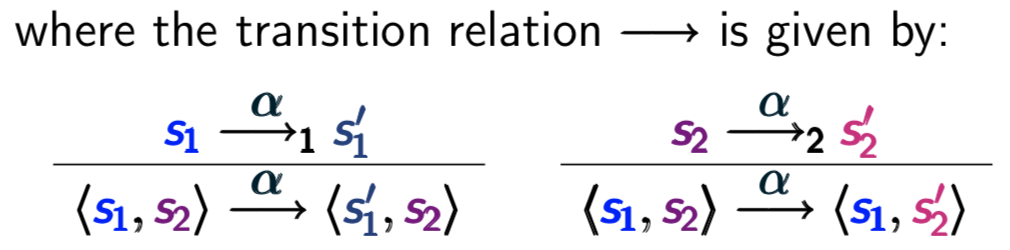
\includegraphics[scale=0.35]{T1T2}
	\end{figure}
\end{multicols}
\noindent
L'operatore di \textit{Interleaving} fallisce per azioni dipendenti, portando a stati inconsistenti.\\
Per questo motivo viene introdotta la \textit{\textbf{Mutua Esclusione}} attraverso i semafori.



\chapter*{Linear Time Properties}
\addcontentsline{toc}{chapter}{Linear Time Properties}
\textit{\textbf{Execution fragment}}: seq. di transizioni infinita ($s_0 \rightarrow^{\alpha_0} s_1 \rightarrow^{\alpha_1} \dots$) o finita ($s_0 \rightarrow^{\alpha_0} s_1 \rightarrow^{\alpha_1} \dots \rightarrow^{\alpha_{n-1}} s_n$).

\noindent
\textit{\textbf{Path fragment}}: sequenza di stati infinita ($\pi = s_0 s_1 s_2\dots$) o finita ($\pi = s_0 s_1 s_2\dots s_n$).\\
Queste possono essere \textit{massimali} se sono infinite oppure finiscono in uno stato terminale.\\\\
\textit{\textbf{Paths}}$(\mathcal{T})$ = insieme dei percorsi massimali, partendo dallo stato iniziale.\\
\textit{\textbf{Paths}}$(s)$ = insieme dei percorsi massimali, partendo dallo stato $s$.\\
\textit{\textbf{Paths}}$_{fin}(s)$ = insieme dei percorsi finiti, partendo dallo stato $s$.\\
\textit{\textbf{Traces}} = sequenza di insiemi di proposizioni atomiche (assumendo che non ci siano stati terminali).\\
\textit{\textbf{Traces}} $(\mathcal{T}) = \{$ trace$(\pi): \pi \in$ Paths$(\mathcal{T})\} \subseteq (2^{AP})^\omega$\\
\textit{\textbf{Traces}}$_{fin} (\mathcal{T}) = \{$ trace$(\hat{\pi}): \hat{\pi} \in$ Paths$_{fin}(\mathcal{T})\} \subseteq (2^{AP})^*$


\section*{Safety}
\addcontentsline{toc}{section}{Safety}
\textit{\textbf{LT Property} (senza stati terminali)}: è un linguaggio $E$ di infinite parole su un alfabeto $\Sigma = 2^{AP}$ con $E \subseteq (2^{AP})^\omega$\\
$\mathcal{T} \vDash E \text{ ~iff~ } Traces(\mathcal{T}) \subseteq E$ ~~~~~~~~~~~~~~~~~~ $s \vDash E \text{ ~iff~ } Traces(s) \subseteq E$\\
\textit{\textbf{Safety} (Mutex)}: su un'insieme infinito di parole, si vogliono evitare situazioni di inconsistenza e deadlock. Abbiamo degli \textit{invarianti} che definiscono le proprietà da non violare. Non ci devono essere \textit{bad prefix} (pay, drink, drink).\\
\textit{\textbf{prefix}}$(\sigma) = $ insieme di prefissi di $\sigma$ non vuoti.\\
\textit{\textbf{prefix}}$(E) = \bigcup_{\sigma \in E} pref(\sigma)$.\\
\textit{\textbf{Prefix closure}}: sono i prefissi che sono accettati dal linguaggio. ~~~$cl(E) = \{ \sigma \in (2^{AP})^\omega : pref(\sigma) \subseteq pref(E) \}$.\\
\textit{\textbf{Teorema}}: $E$ è una \textit{safety property} se e solo se $cl(E) = E$.


\section*{Liveness}
\addcontentsline{toc}{section}{Liveness}
\textit{\textbf{Liveness} (Live)}: si vogliono evitare situazioni di starvation (da wait possono sempre andare in crit).\\
$E$ è chiamata \textit{\textbf{liveness property}} se ogni parola finita può essere estesa ad una parola infinita in $E$. ~~$pref(E) = (2^{AP})$


\section*{Fairness}
\addcontentsline{toc}{section}{Fairness}
Dato $\rho = s_0 \rightarrow^{a_0} s_1 \rightarrow^{a_1} s_2 \rightarrow^{a_2} \dots$, un frammento infinito di esecuzione:\\
\textit{\textbf{Unconditional Fairness}}: $\stackrel{\infty}{\exists} i \geq 0. ~\alpha_i \in A$\\
$\rho$ è \textit{unconditional A-fair} se l'azione $A$ viene eseguita infinitamente spesso.\\
Ogni processo ottiene il suo turno infinitamente spesso.\\\\
\textit{\textbf{Strong Fairness}}: $\stackrel{\infty}{\exists} i \geq 0. ~A \cap Act(s_i) \neq \emptyset ~\Longrightarrow~ \stackrel{\infty}{\exists} i \geq 0. ~\alpha_i \in A$\\
Ogni processo che è abilitato infinitamente spesso, ottiene il suo turno infinitamente spesso.\\
$\rho$ non è \textit{strongly A-fair} se:
\begin{itemize}
	\item nessuna azione $A$ viene eseguita da un certo momento;
	\item l'azione $A$ è abilitata infinite volte.
\end{itemize}
\textit{\textbf{Weak Fairness}}: $\stackrel{\infty}{\forall} i \geq 0. ~A \cap Act(s_i) \neq \emptyset ~\Longrightarrow~ \stackrel{\infty}{\exists} i \geq 0. ~\alpha_i \in A$\\
Ogni processo che è continuamente abilitato, da un certo momento in poi, ottiene il suo turno infinitamente spesso.\\
$\rho$ non è \textit{weak A-fair} se:
\begin{itemize}
	\item nessuna azione $A$ viene eseguita da un certo momento;
	\item l'azione $A$ è continuamente abilitata da un certo punto in poi.
\end{itemize}
\textit{\textbf{Unconditionally A-fair}} $\Rightarrow$ \textit{\textbf{Strongly A-fair}} $\Rightarrow$ \textit{\textbf{Weakly A-fair}}



\chapter*{Linear Temporal Logic}
\addcontentsline{toc}{chapter}{Linear Temporal Logic}
\begin{multicols}{2}
	\noindent
	\textit{\textbf{Next operator}}: $\bigcirc a$ significa che vale $a$ solo nell'istante successivo. Self Duality: $\bigcirc \lnot \phi = \lnot \bigcirc \phi$\\
	\textit{\textbf{Until operator}}: $a \bigcup b$ significa che continua a valere $a$ fino ad un certo punto in cui varrà $b$ e non più $a$.
	\columnbreak
	\begin{figure}[H]
		\centering
		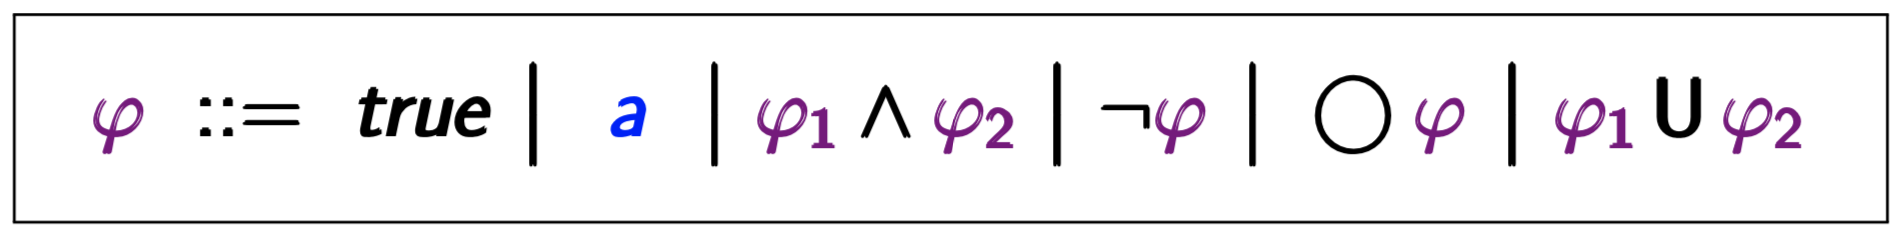
\includegraphics[scale=0.2]{LTL}
	\end{figure}
\end{multicols}
\noindent
\textit{\textbf{Diamond operator}}: $\Diamond \phi= true \bigcup \phi$ ~~significa ad un certo punto varrà $\phi$ almeno una volta.\\
\textit{\textbf{Box operator}}: $\Box \phi = \lnot \Diamond \lnot \phi$ ~~significa che varrà sempre $\phi$\\
\textit{\textbf{Weak until}}: $\phi ~\mathcal{W}~ \psi \equiv (\phi \bigcup \psi) \lor \Box \phi$\\\\
\textit{\textbf{Spesso infinite volte}}: $\Box \Diamond \phi$\\
\textit{\textbf{Prima o poi sempre}}: $\Diamond \Box \phi$\\
\textit{\textbf{Words}}$(\phi) = \{\sigma \in (2^{AP})^\omega: \sigma \vDash \phi \}$\\
\textit{\textbf{Expansion Law}}: $\psi_1 \bigcup \psi_2 \equiv \psi_2 \lor (\psi_1 \land \bigcirc(\psi_1 \bigcup \psi_2))$\\

\hrule

\begin{multicols}{2}
	\begin{figure}[H]
		\centering
		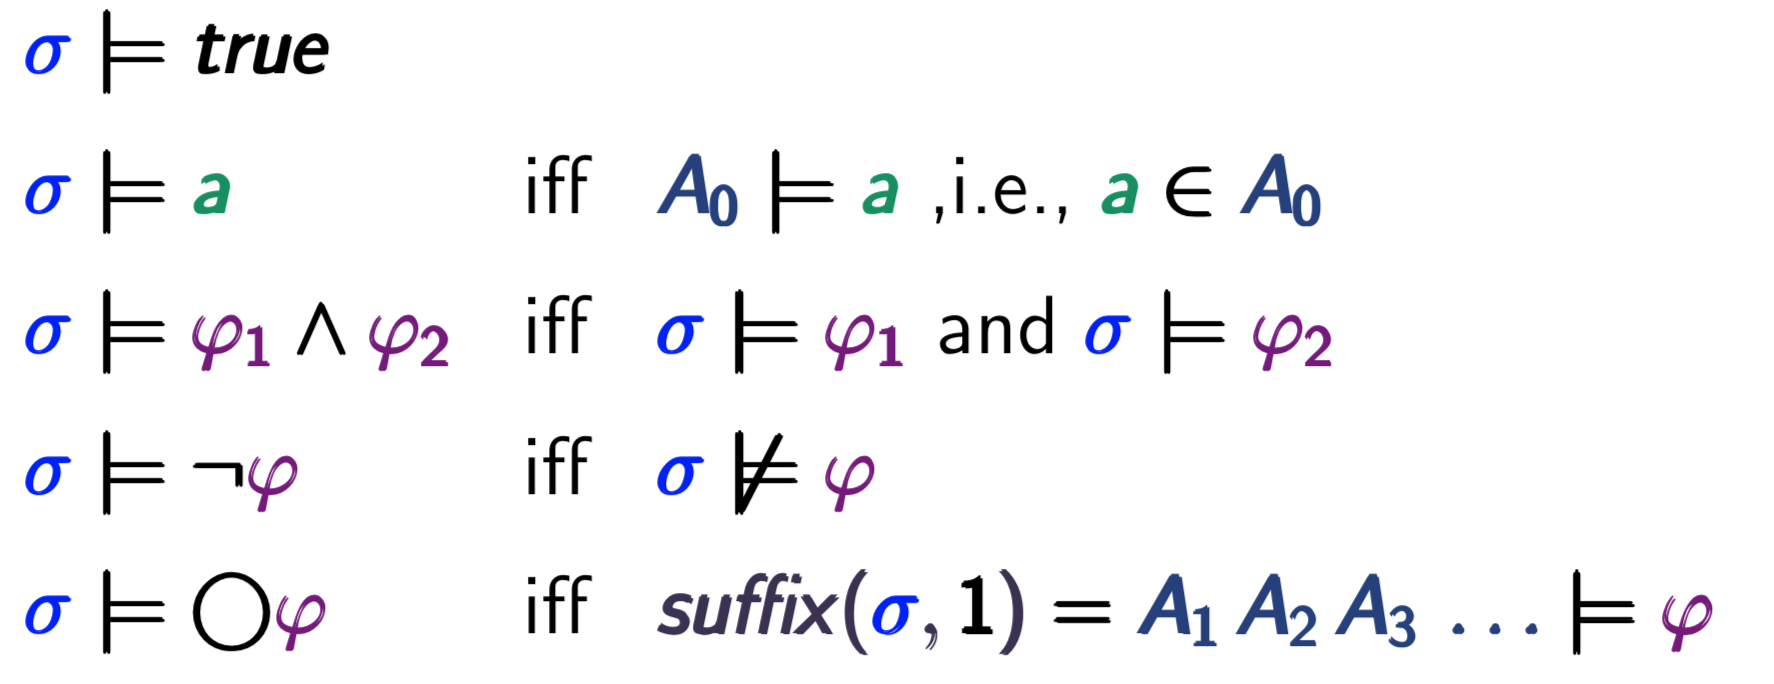
\includegraphics[scale=0.18]{A1}
	\end{figure}
	\begin{figure}[H]
		\centering
		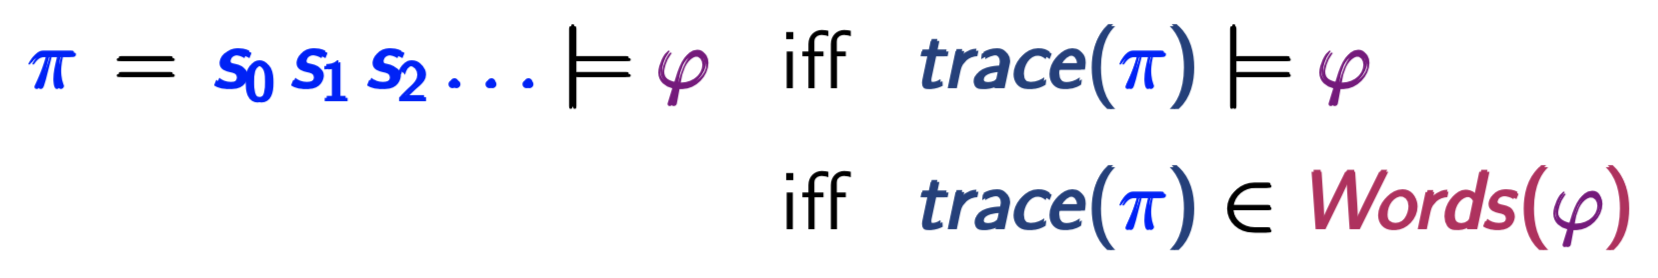
\includegraphics[scale=0.17]{A3}
	\end{figure}
	\columnbreak
	\begin{figure}[H]
		\centering
		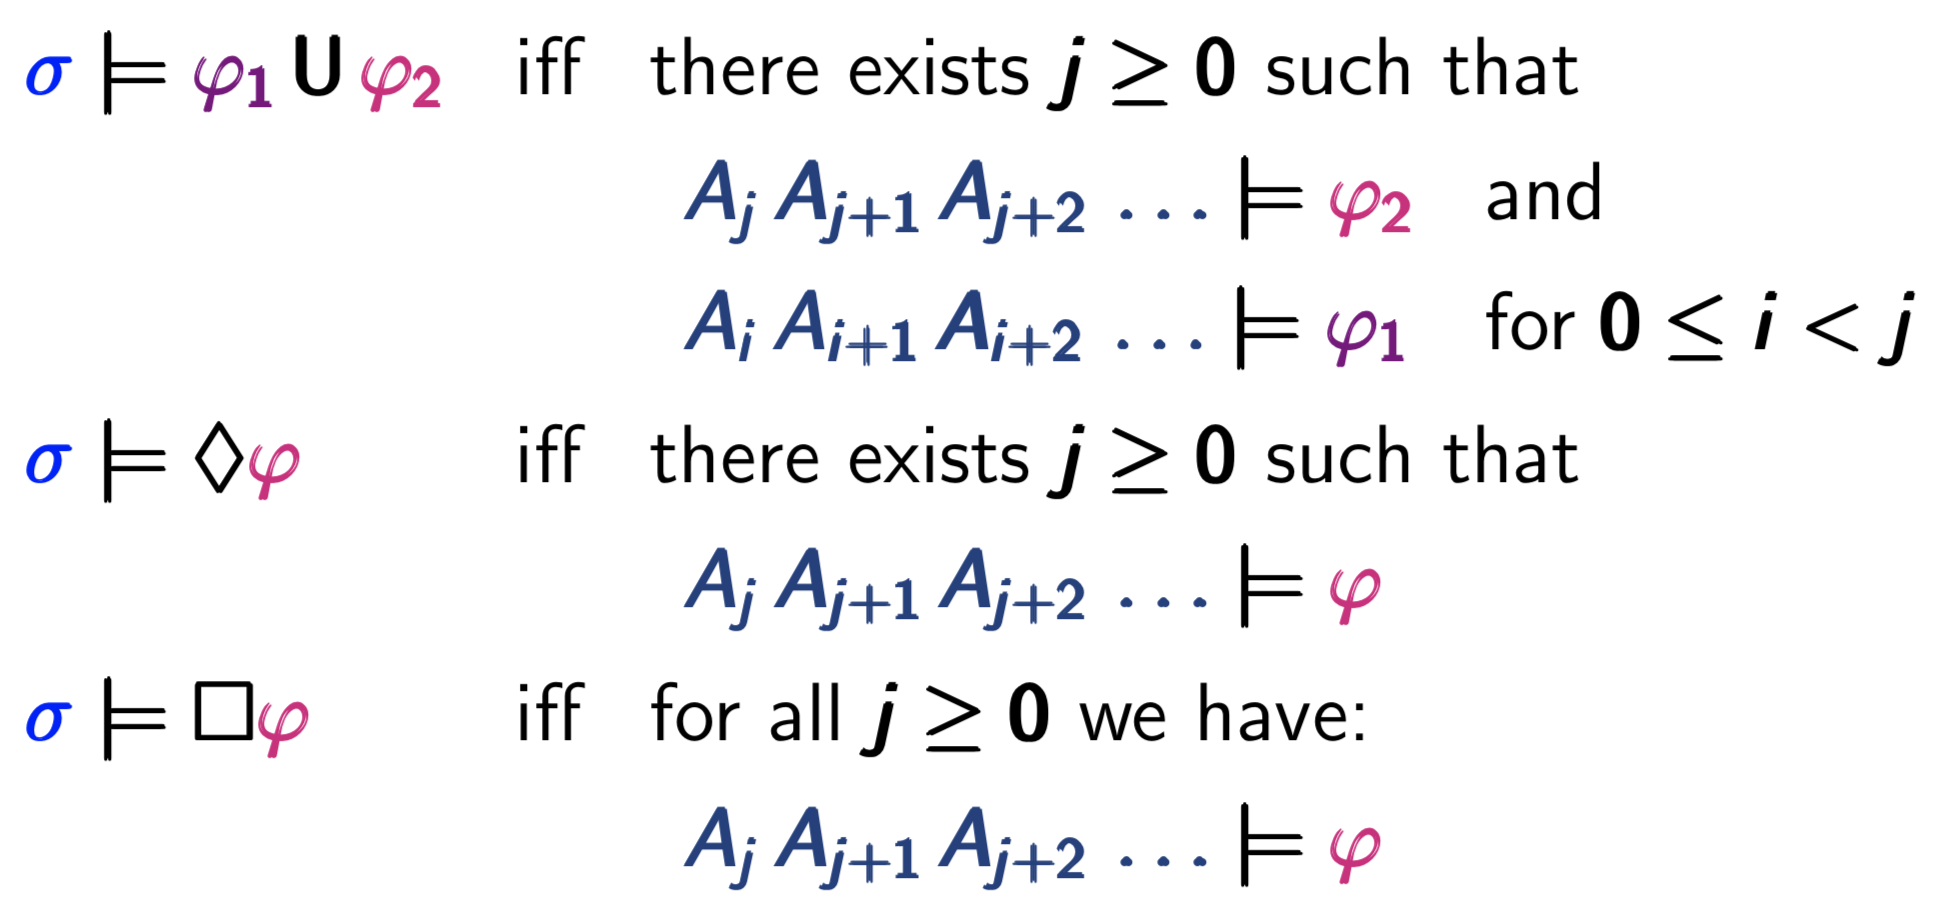
\includegraphics[scale=0.21]{A2}
	\end{figure}
\end{multicols}

\hrule

\begin{multicols}{2}
	\begin{figure}[H]
		\centering
		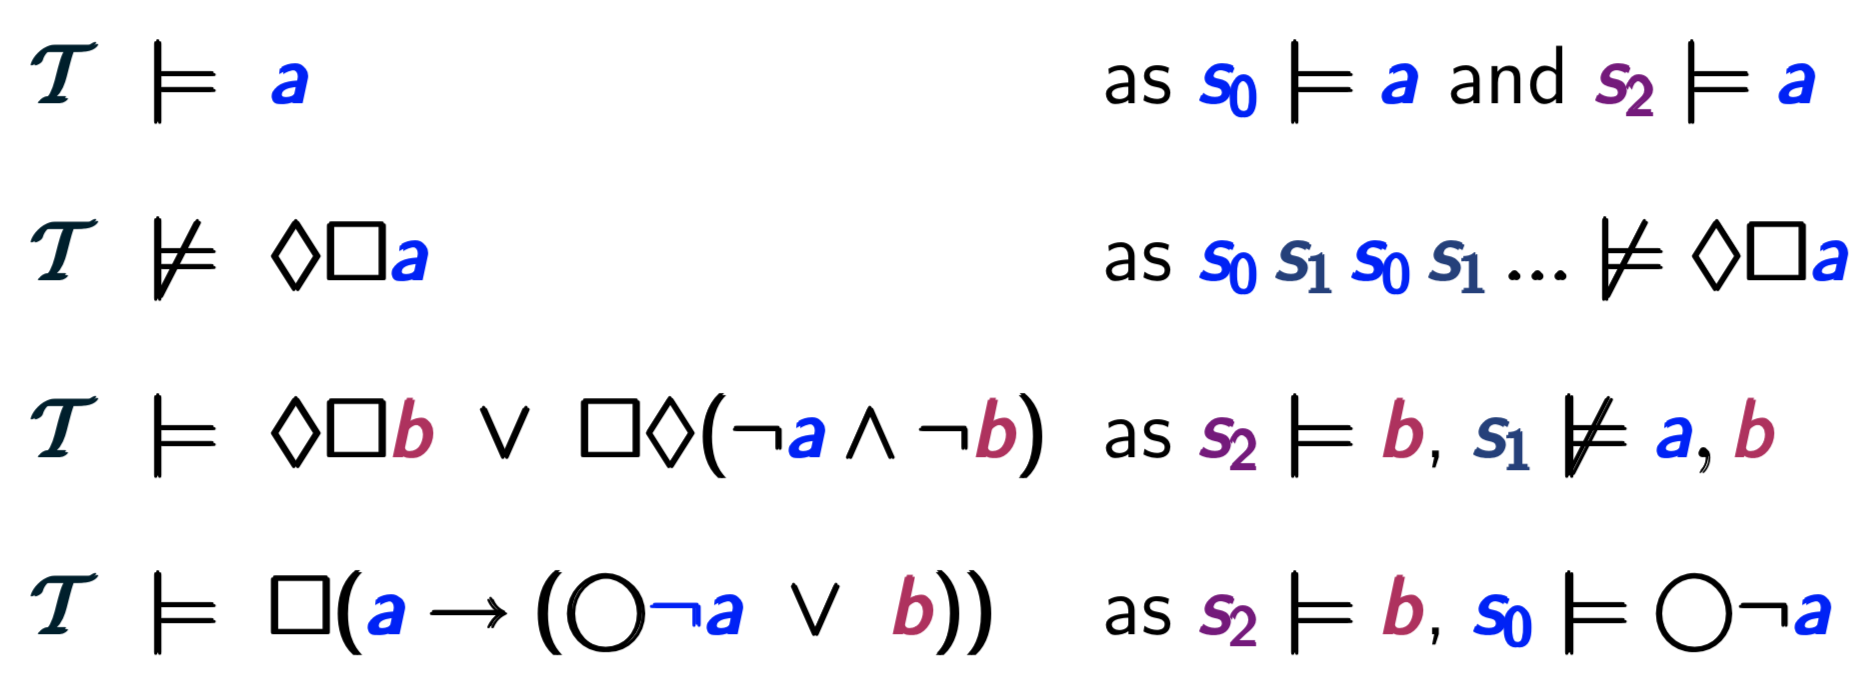
\includegraphics[scale=0.15]{B1}
	\end{figure}
	\columnbreak
	\begin{figure}[H]
		\centering
		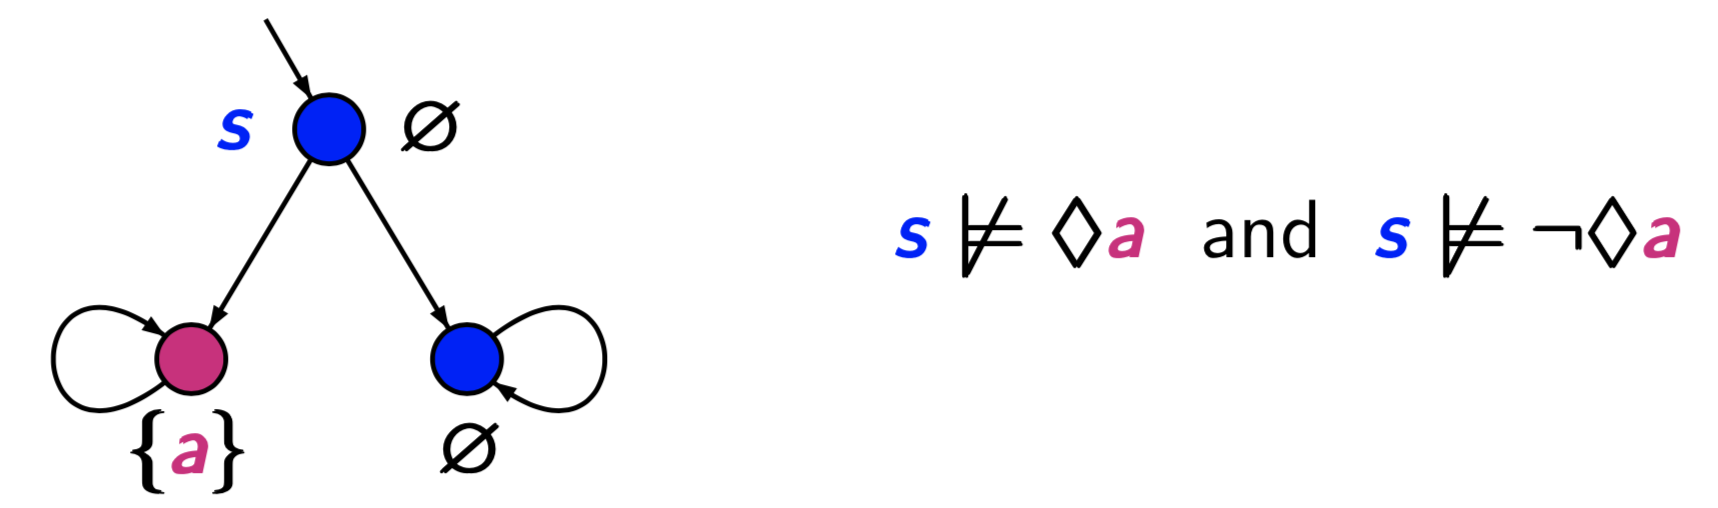
\includegraphics[scale=0.2]{B2}
	\end{figure}
\end{multicols}

\hrule

\begin{multicols}{2}
	\begin{figure}[H]
		\centering
		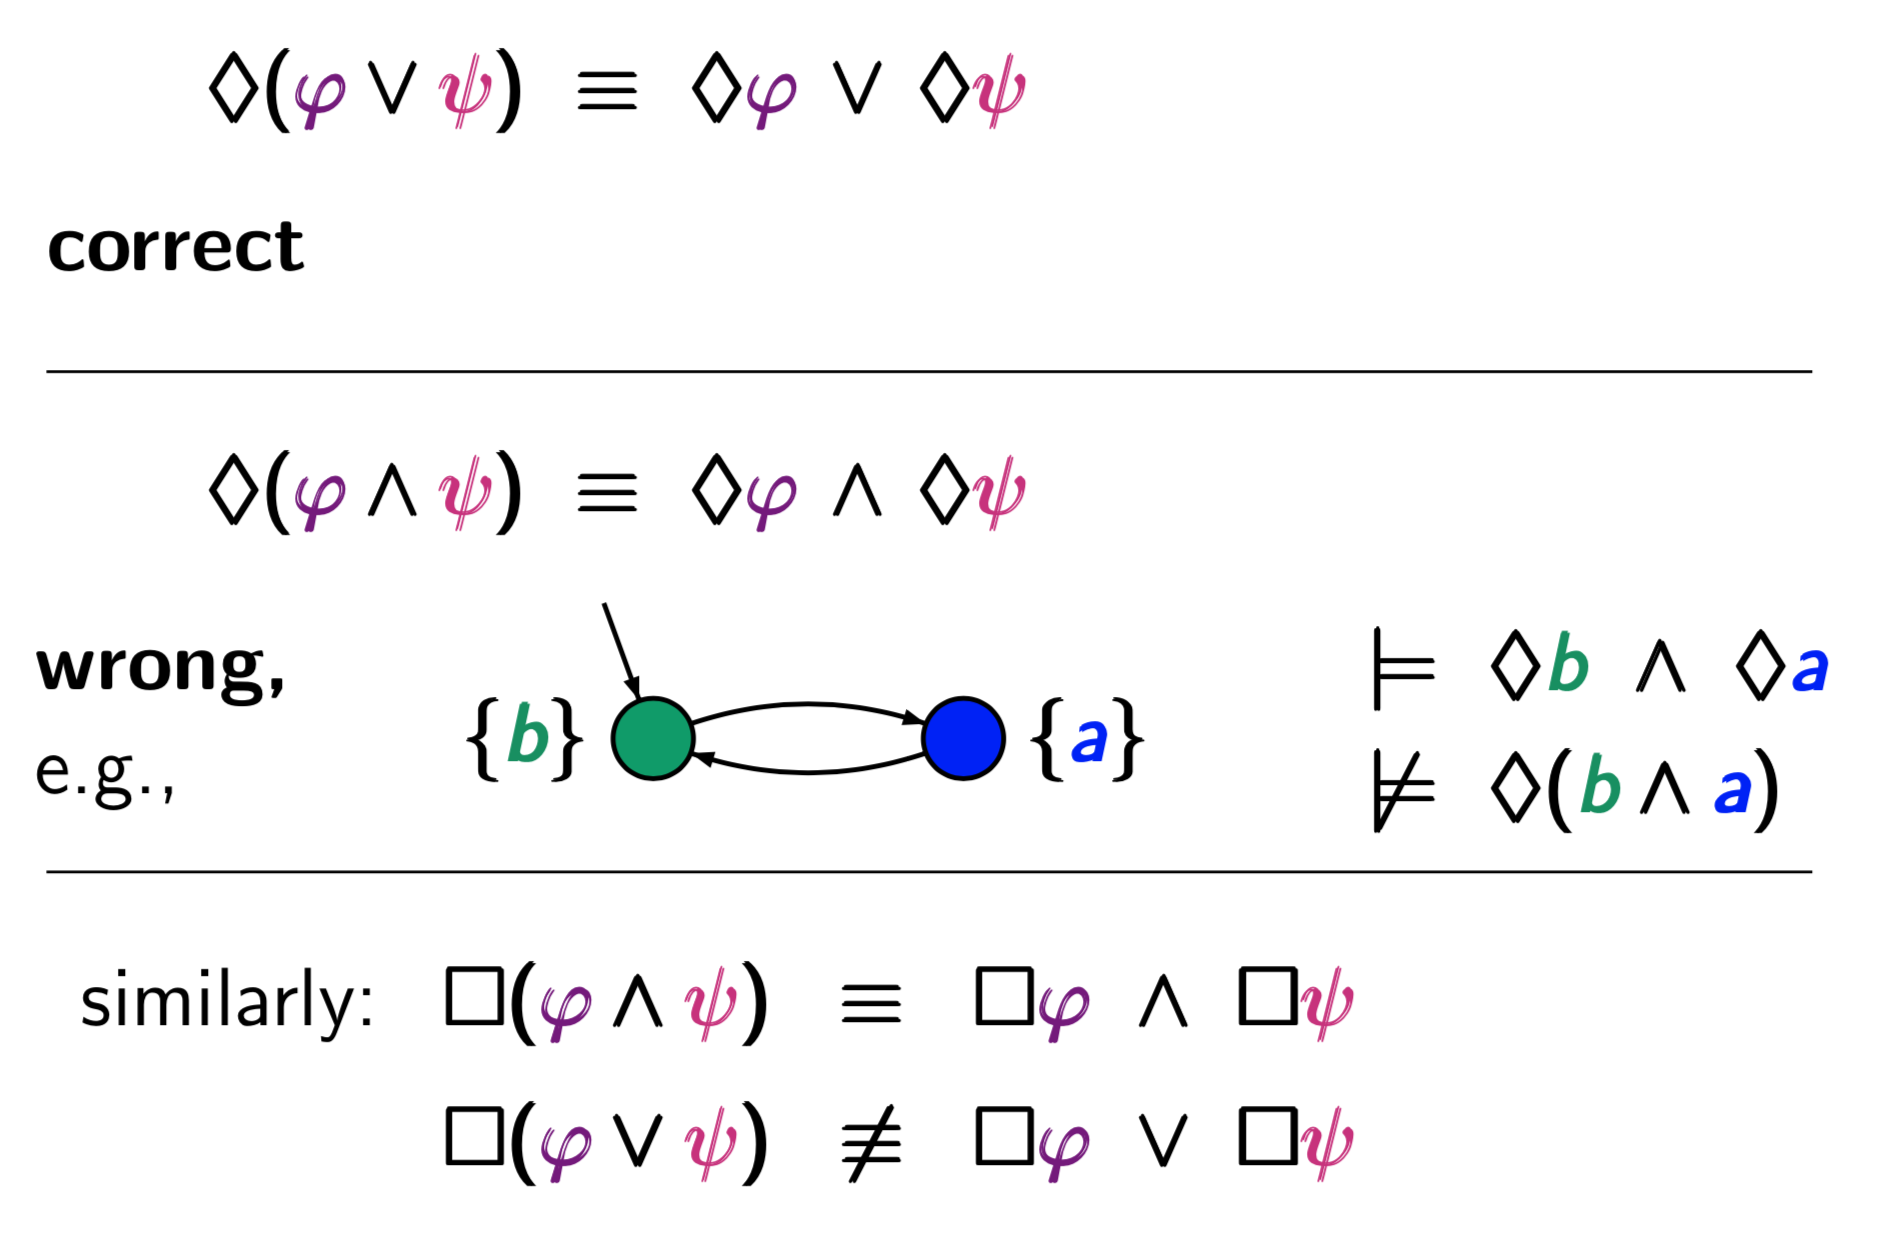
\includegraphics[scale=0.15]{C1}
	\end{figure}
	\columnbreak
	\begin{figure}[H]
		\centering
		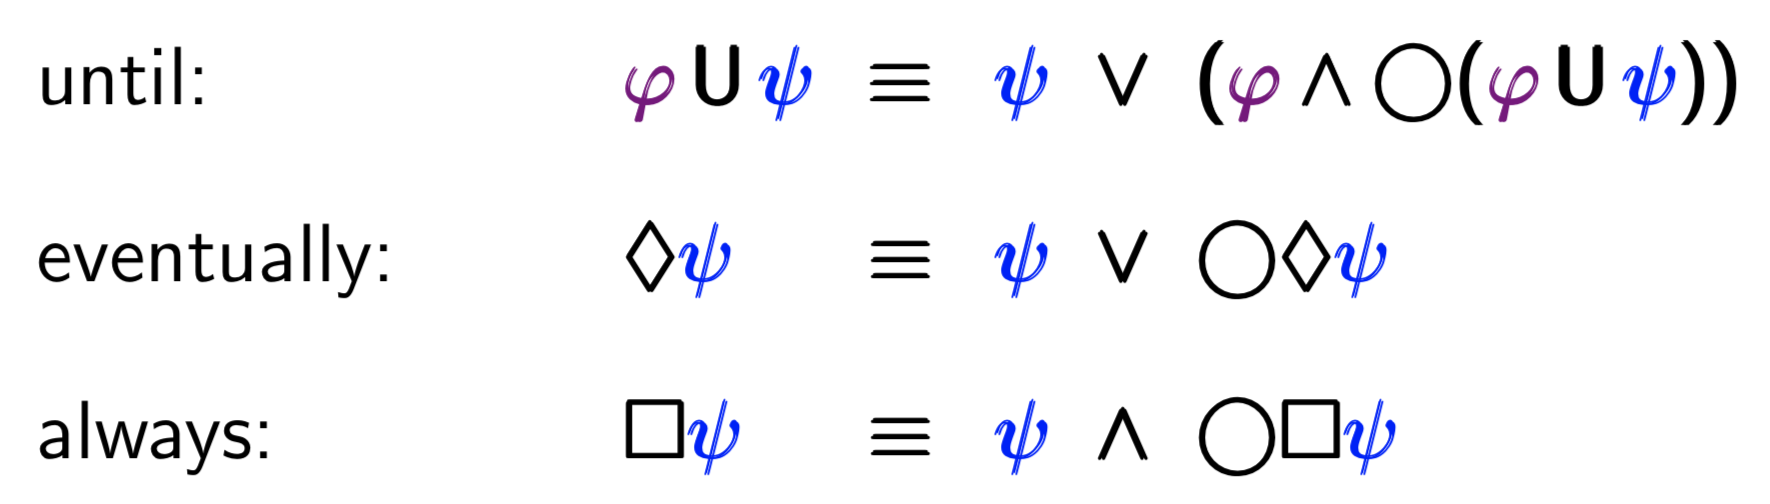
\includegraphics[scale=0.2]{C2}
	\end{figure}
\end{multicols}

\noindent
\textit{\textbf{Positive Normal Form} (PNF)}: proprietà per eliminare il \textit{not} da una formula, trasformandola.
\begin{multicols}{2}
\noindent
$\lnot \Diamond \phi$ ~~diventa~~ $\Box \lnot \phi$\\
$\lnot \Box \phi$  ~~diventa~~ $\Diamond \lnot \phi$\\
$\lnot \bigcirc \phi$ ~~diventa~~ $\bigcirc \lnot \phi$
\columnbreak
\begin{figure}[H]
	\centering
	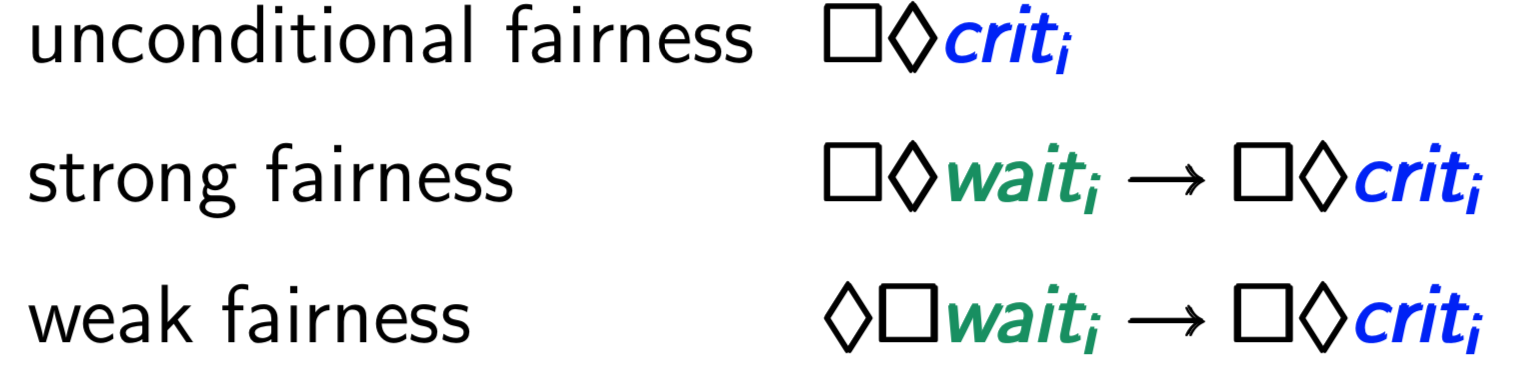
\includegraphics[scale=0.25]{D1}
\end{figure}
\end{multicols}


\section*{Model Checking}
\addcontentsline{toc}{section}{Model Checking}
L'idea di base consiste nel confutare $\mathcal{T} \vDash \phi$ cercando un path $\pi$ in $\mathcal{T}$ tale che $\pi \vDash \lnot \phi$\\\\
\textit{\textbf{NBA} (Non-Determinist B\"{u}chi Automata)} $\mathcal{A} = (Q, \Sigma, \delta Q_0, F)$
\begin{itemize}
	\item $Q$ insieme finito di stati;
	\item $\Sigma$ alfabeto;
	\item $\delta: Q \times \Sigma \rightarrow 2^Q$ relazione di transizione;
	\item $Q_0 \subseteq Q$ insieme di stati iniziali;
	\item $F \subseteq Q$ insieme di stati finali, anche chiamati stati accettanti.
\end{itemize}


\noindent
Dato $\pi = q_0 q_1 q_2 \dots$ dove $q_0 \in Q_0$ e $q_{i+1} \in \delta(q_i, A_i)$ per $i \geq 0$, un path $\pi$ è accettante se $\stackrel{\infty}{\exists} i \in \mathbb{N}. ~q_i \in F$\\
$\mathcal{L}_\omega(\mathcal{A}) = $ insieme di parole infinite su $\Sigma$ che hanno un path/run accettante in $\mathcal{A}$.\\\\
\textit{\textbf{GNBA} (Generalized Non-Determinist B\"{u}chi Automata)} $\mathcal{G} = (Q, \Sigma, \delta, Q_0, \mathcal{F})$
\begin{itemize}
	\item $Q, \Sigma, \delta, Q_0$ sono come in NBA;
	\item $\mathcal{F} \subseteq 2^Q$ è un set di set accettanti, tali che $\mathcal{F} = \{ F_{\phi_1 \bigcup \phi_2}: \phi_1 \bigcup \phi_2 \in cl(\phi) \}$.
\end{itemize}

\noindent
Una run $\pi = q_0 q_1 q_2 \dots$ è accettante se ogni set accettante è visitato infinitamente spesso. ~$\forall F \in \mathcal{F} ~~\stackrel{\infty}{\exists} i \in \mathbb{N}. ~q_i \in F$.\\
$\mathcal{L}_\omega(\mathcal{G}) = \{\sigma \in \Sigma^\omega: \sigma$ ha una run accettante in $\mathcal{G} \}$\\
\begin{multicols}{2}
	\noindent
	Per ogni \textit{GNBA} $\mathcal{G}$ esiste un \textit{NBA} $\mathcal{A}$ corrispondente con $\mathcal{L}_\omega(\mathcal{G}) = \mathcal{L}_\omega(\mathcal{A})$.\\\\
	Per ogni formula \textit{LTL} $\phi$ su AP c'è un \textit{NBA} $\mathcal{A}$ su un alfabeto $2^{AP}$ tale che:
	\begin{itemize}
		\item \textit{Words}$(\phi) = \mathcal{L}_\omega(\mathcal{A})$
		\item size $(\mathcal{A}) = \mathcal{O}(exp (|\phi|))$
	\end{itemize}
	\columnbreak
	\begin{figure}[H]
		\centering
		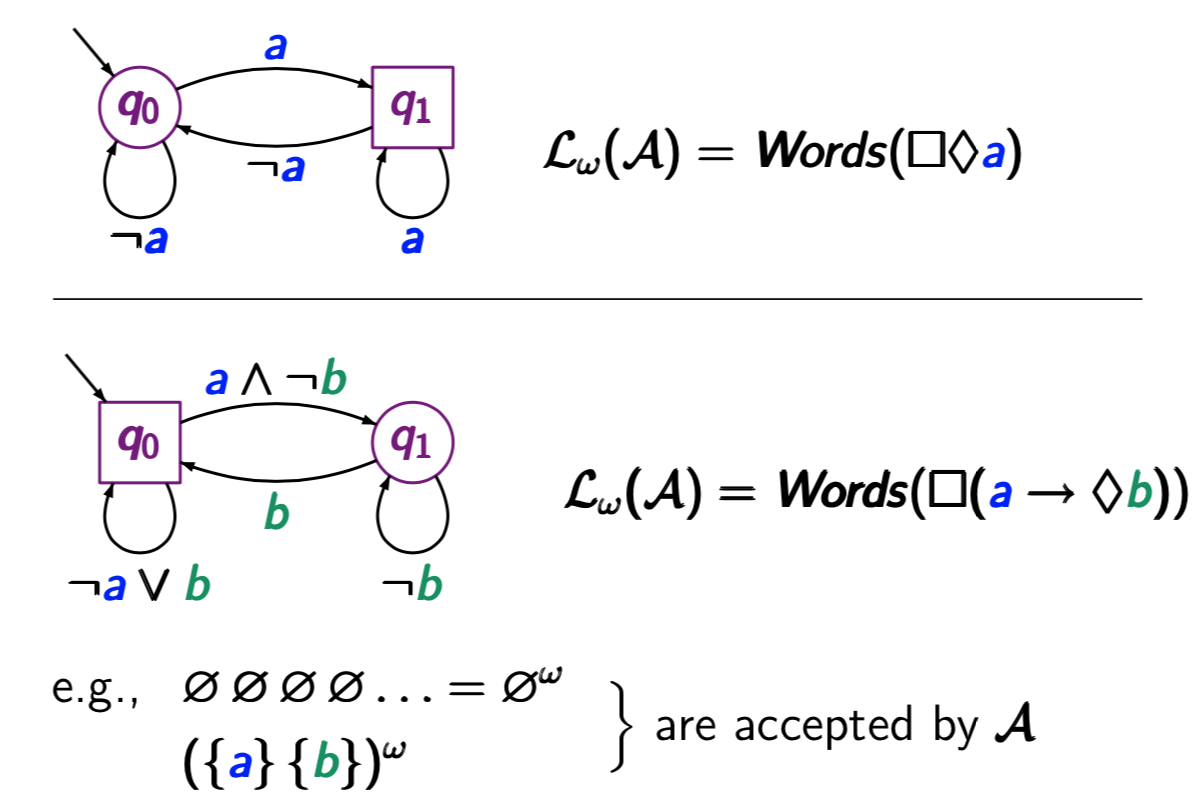
\includegraphics[scale=0.24]{NBA}
	\end{figure}
\end{multicols}

\noindent
\textit{\textbf{Persistence checking}}: $\mathcal{T} \otimes \mathcal{A} \vDash \Diamond \Box \lnot F$\\\\
\textit{\textbf{From LTL to GNBA}}: si passa dalle $A_0 A_1 \dots \in Words(\phi)$ a $B_0 B_1 \dots$ run accettanti, con $B_i = \{\psi \in cl(\phi): A_i A_{i+1}\dots \vDash \psi \}$. Sappiamo che $cl(\phi)$ sono le sottoformule di $\phi$ e i loro negati.\\
Sia $B \subseteq cl(\phi)$. $B$ è elementare se:
\begin{itemize}
	\item $B$ è consistente, cioé se $\psi \in B$ allora $\lnot \psi \notin B$
	\item $B$ è massimamente consistente, cioé se $\psi \in cl(\phi)\backslash B$ allora $\lnot \psi \in B$
	\item $B$ è localmente consistente rispetto all'\textit{until} $\bigcup$, cioé se $\psi_1 \bigcup \psi_2 \in B$ e $\lnot \psi_2 \in B$ allora $\lnot \psi_1 \notin B$
\end{itemize}


\section*{Fairness in LTL e in CTL}
\addcontentsline{toc}{section}{Model Checking}
\begin{multicols}{2}
	\noindent
	\textit{\textbf{LTL}}:
	\begin{itemize}
		\item \textit{Unconditional fairness}: $\Box \Diamond \phi$
		\item \textit{Strong fairness}: $\Box \Diamond \psi \rightarrow \Box \Diamond \phi$
		\item \textit{Weak fairness}: $\Diamond \Box \psi \rightarrow \Box \Diamond \phi$
	\end{itemize}
\columnbreak
	\noindent
\textit{\textbf{CTL}}:
	\begin{itemize}
		\item \textit{Unconditional fairness}: $\forall \Box \forall \Diamond \phi$
		\item \textit{Strong fairness}: $\forall \Box \forall \Diamond \psi \rightarrow \forall \Box \forall \Diamond \phi$
		\item \textit{Weak fairness}: non c'è in CTL (dim. sotto).
	\end{itemize}
\end{multicols}



\chapter*{Computation Tree Logic}
\addcontentsline{toc}{chapter}{Computation Tree Logic}
\begin{multicols}{2}
	\noindent
$\forall \bigcirc \phi =$ per ogni stato figlio vale $\phi$;\\
$\exists \bigcirc \phi =$ esiste un figlio in cui vale $\phi$.\\
$\forall \Box \phi =$ per ogni computazione (branch) e per ogni stato della computazione vale $\phi$.\\
$\forall \Diamond \phi =$ per ogni computazione prima o poi vale $\phi$.\\
$\exists \Box \phi =$ esiste una computazione in cui, per ogni stato, vale $\phi$.\\
$\exists \Diamond \phi =$ esiste una computazione in cui vale in un solo stato $\phi$.\\\\
Il quantificatore di esistenza ($\exists$) può essere ricavato attraverso delle operazioni sul quantificatore $\forall$:\\
$\exists \Box A := \lnot\forall \Diamond \lnot A$\\
$\exists \Diamond A := \lnot\forall \Box \lnot A$\\
$\exists \bigcirc A := \lnot\forall \bigcirc \lnot A$\\\\
Un $(UB-)$frame $\langle S, N \rangle$  è un grafo dove $N\subseteq S \times S$ è totale ($\forall s \exists s' ~sNs'$).\\
Un $(UB-)$model $\langle F, V \rangle$  è una coppia dove $F$ è un frame e $V: s\rightarrow 2^{prop}$ è una valutazione.
\columnbreak
\begin{figure}[H]
	\centering
	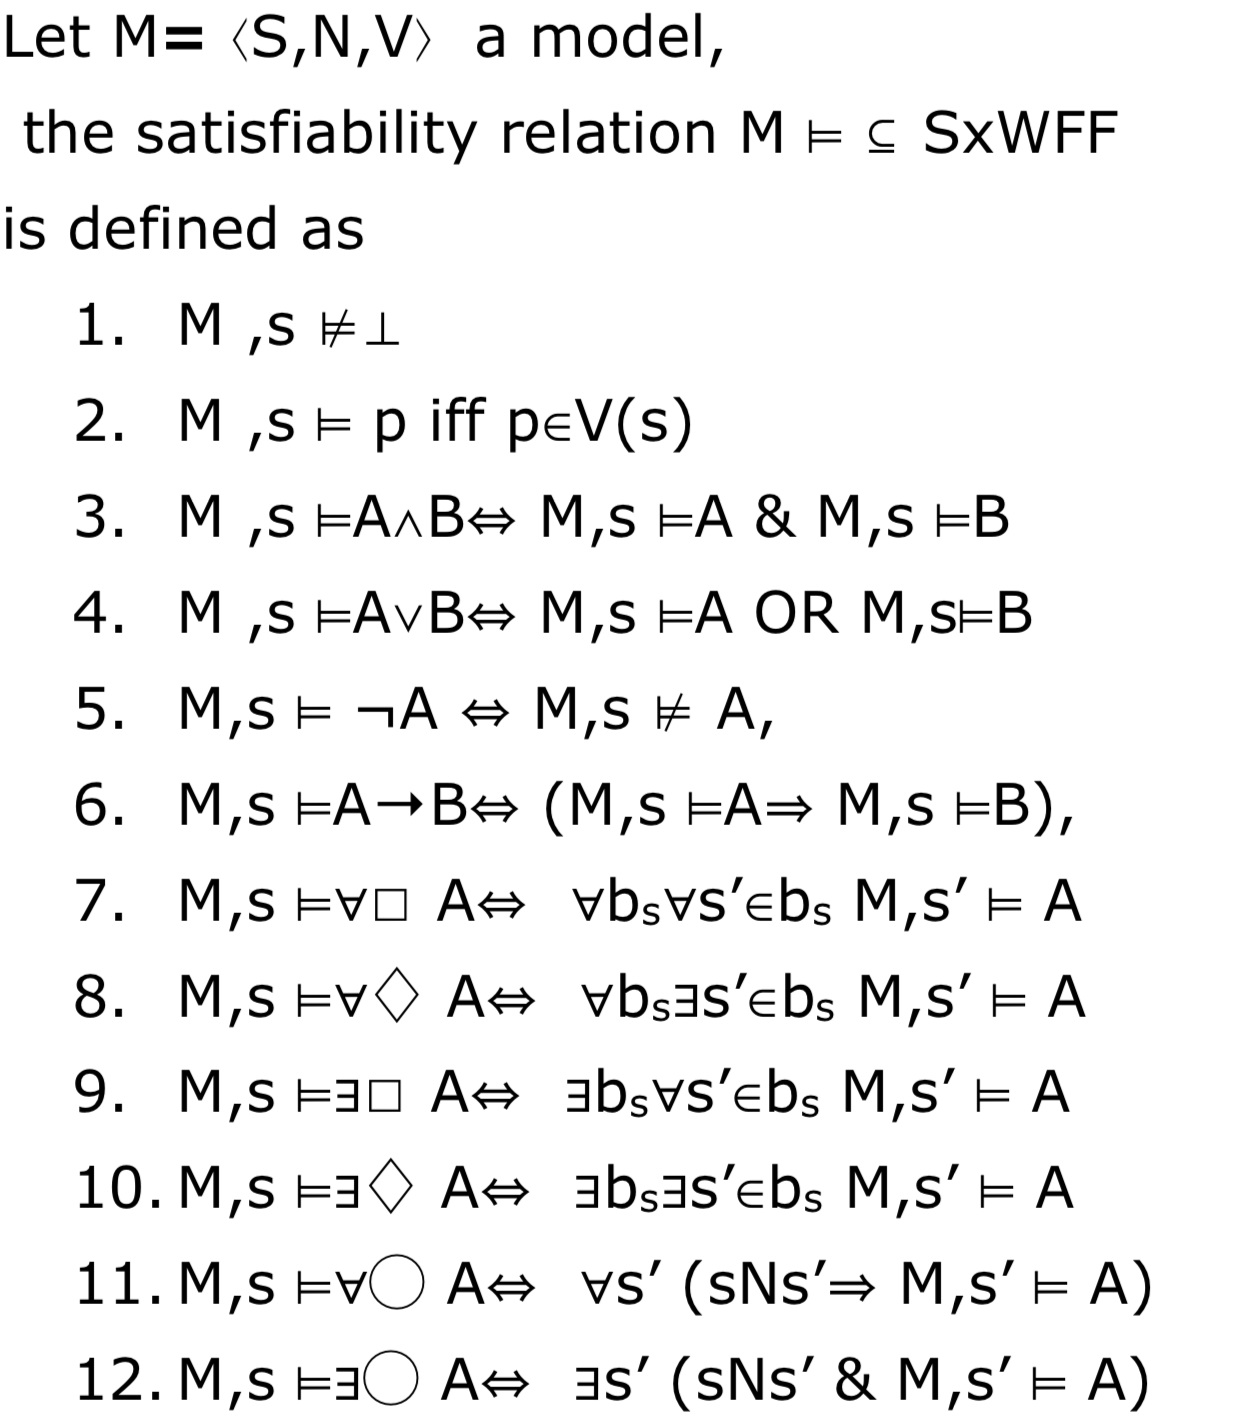
\includegraphics[scale=0.25]{CTL}
\end{figure}
\noindent
Con $s' \in b_s$ si intende un figlio di $s$ che appartiene ad un suo branch.
\end{multicols}

\noindent
Alla semantica $CTL$ si aggiunge l'operatore \textit{Until} $\bigcup$.\\
$M, s \vDash B ~\exists \bigcup A \Leftrightarrow \exists b_s \exists k (M, b_s[k] \vDash A ~\&~ \forall j\in [0, k-1] ~~b_s[j] \vDash B)$\\
$M, s \vDash B ~\forall \bigcup A \Leftrightarrow \forall b_s \exists k (M, b_s[k] \vDash A ~\&~ \forall j\in [0, k-1] ~~b_s[j] \vDash B)$\\\\
$\exists \Diamond \alpha \equiv \text{true} ~\exists \bigcup A$\\
$\forall \Diamond \alpha \equiv \text{true} ~\forall \bigcup A$


\section*{Computation Tree}
\addcontentsline{toc}{section}{Computation Tree}
\begin{multicols}{2}
	\noindent
	Per costruire il \textit{computation tree} di un transition system, è necessario farne l'unfolding. Se ci sono più stati iniziali, si rappresenta un albero per ciascuno stato $s_0$.\\\\	
	$\exists \lnot \Diamond \lnot \phi$ non è una formula CTL (non c'è $\lnot$ nelle path).\\
	$\forall \Box \forall \Diamond$ crit$_1 \land \forall \Box \forall \Diamond$ crit$_2$ (per ogni branch, per ogni stato prima o poi vale crit$_i$; infinitamente spesso).
\columnbreak

$\forall \Box \exists \Diamond$ reset (per ogni branch, prima o poi reset).
	\begin{figure}[H]
		\centering
		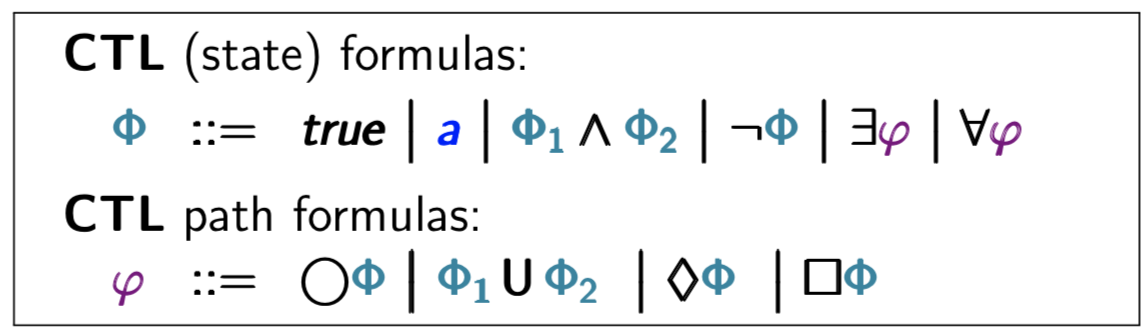
\includegraphics[scale=0.26]{CTL2}
	\end{figure}
\end{multicols}

\begin{multicols}{2}
	\textit{\textbf{Path Formulas}}
	\begin{figure}[H]
		\centering
		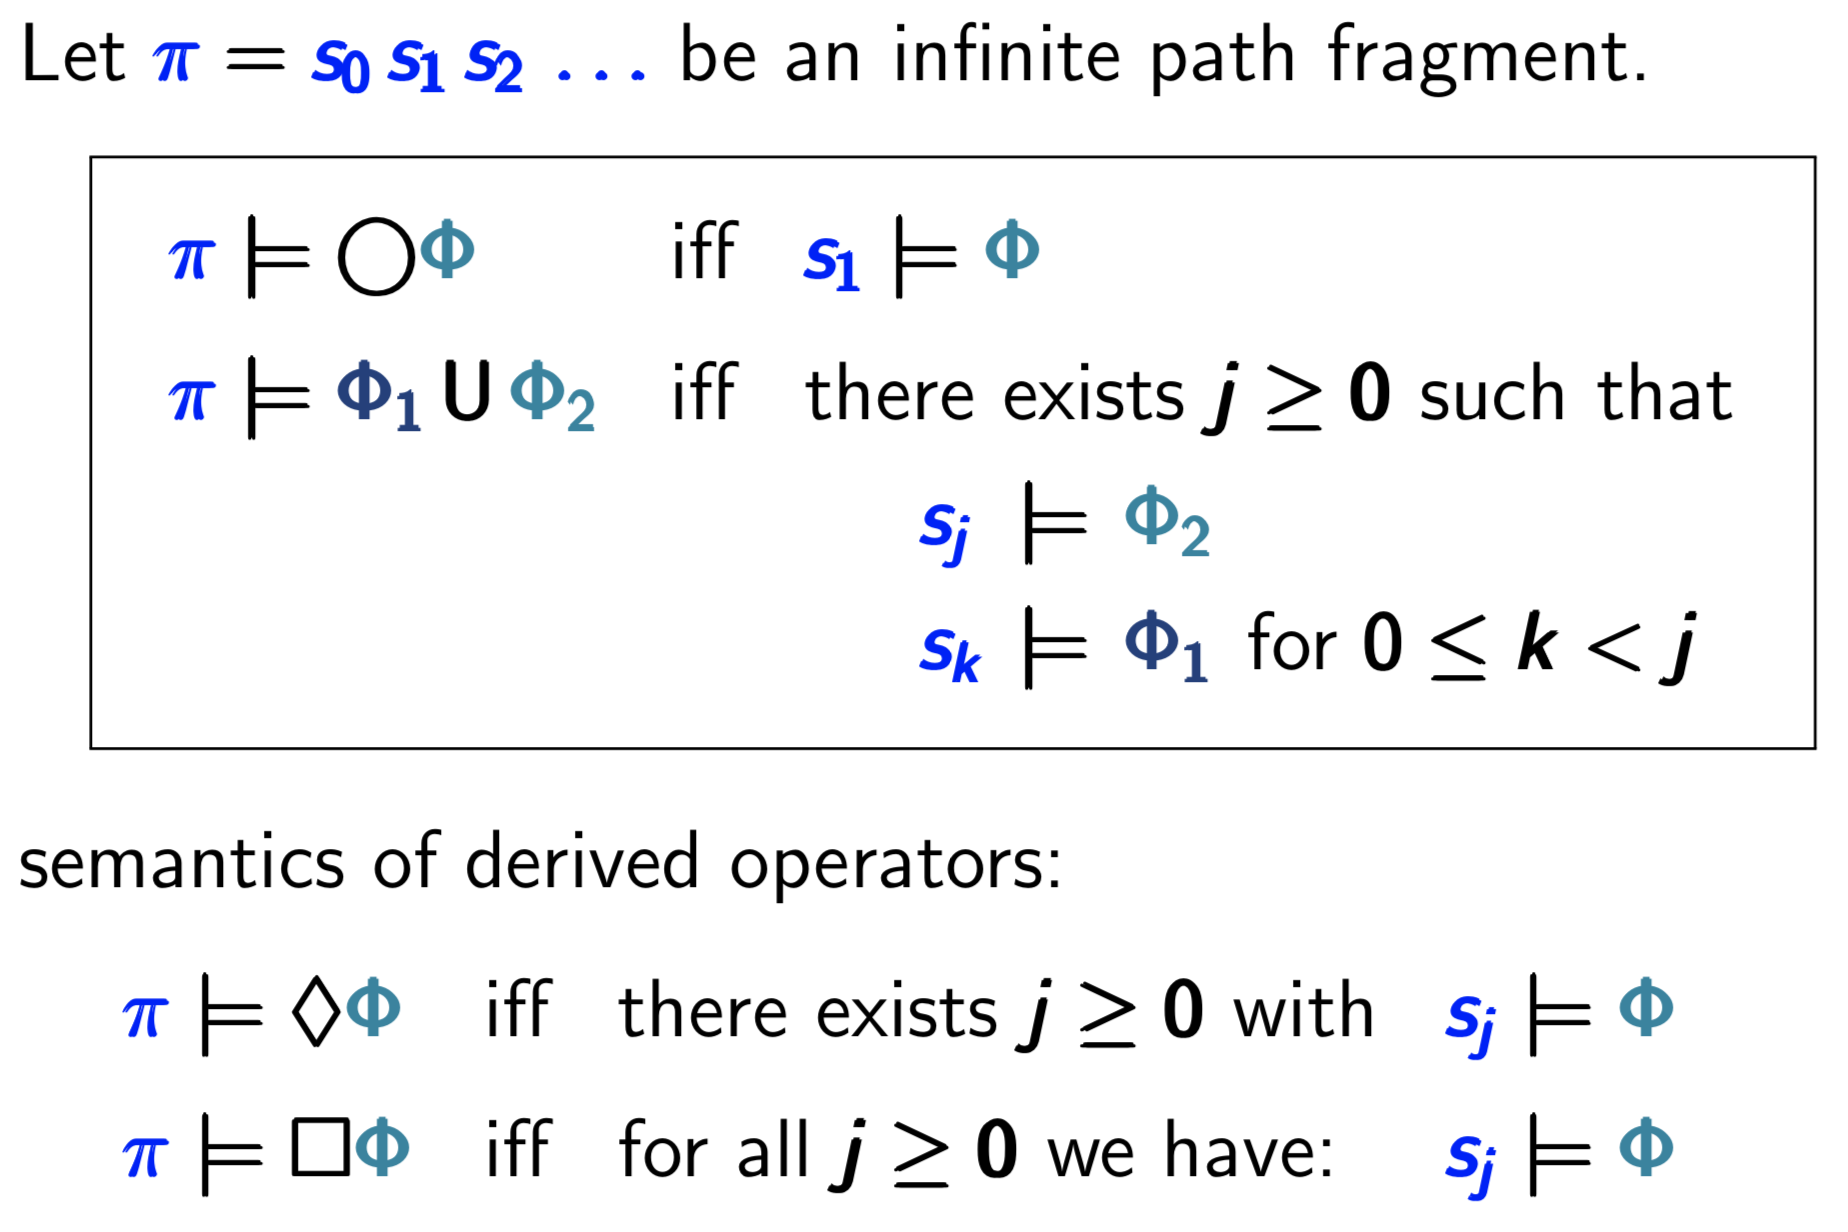
\includegraphics[scale=0.133]{PATH}
	\end{figure}
\columnbreak
	\textit{\textbf{State Formulas}}
	\begin{figure}[H]
		\centering
		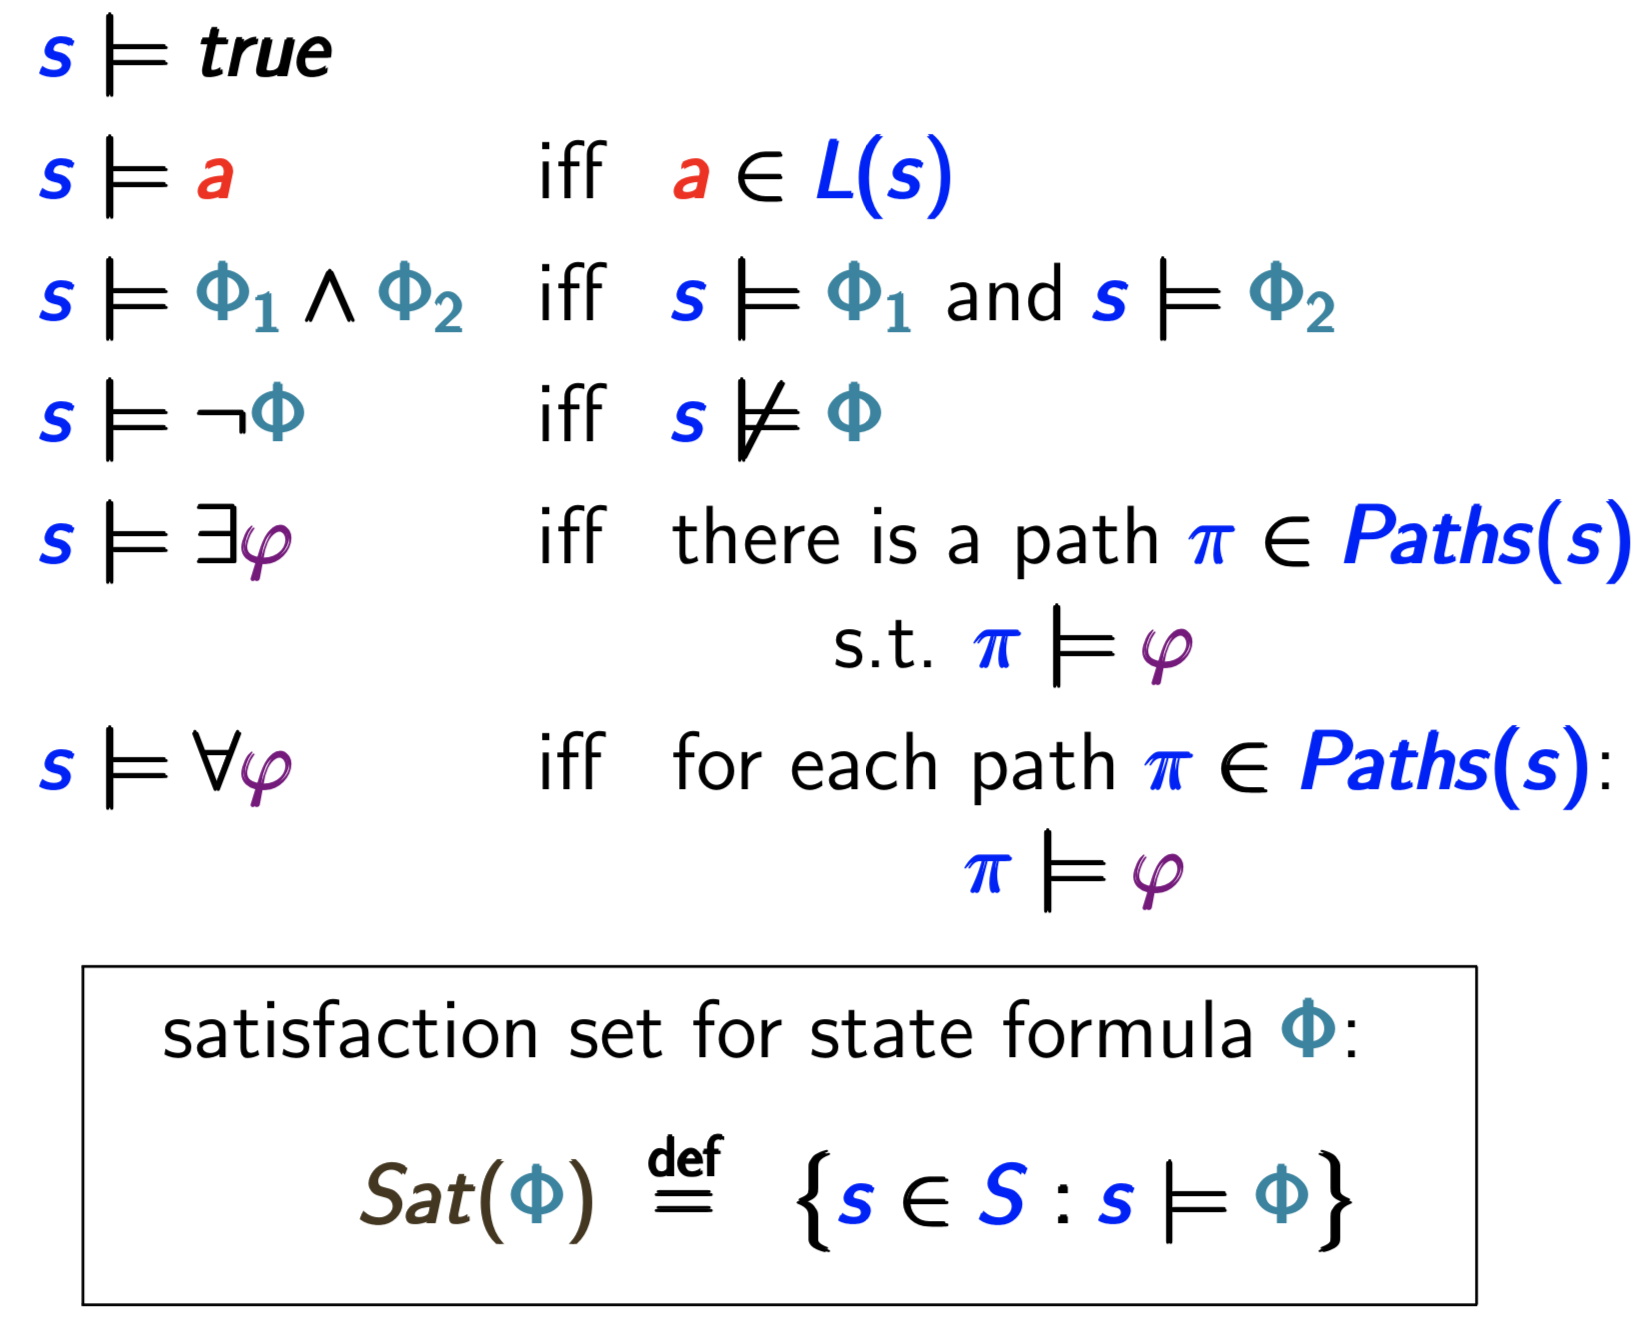
\includegraphics[scale=0.126]{STATE}
	\end{figure}
\end{multicols}

\noindent
$\mathcal{T} \vDash \phi \Leftrightarrow S_0 \subseteq Sat(\phi) \Leftrightarrow s_0 \vDash \phi ~\forall s_0 \in \mathcal{T}$ ~con~ $Sat(\phi) = \{s \in S: s \vDash \phi \}$
\begin{multicols}{3}
	\begin{figure}[H]
		\centering
		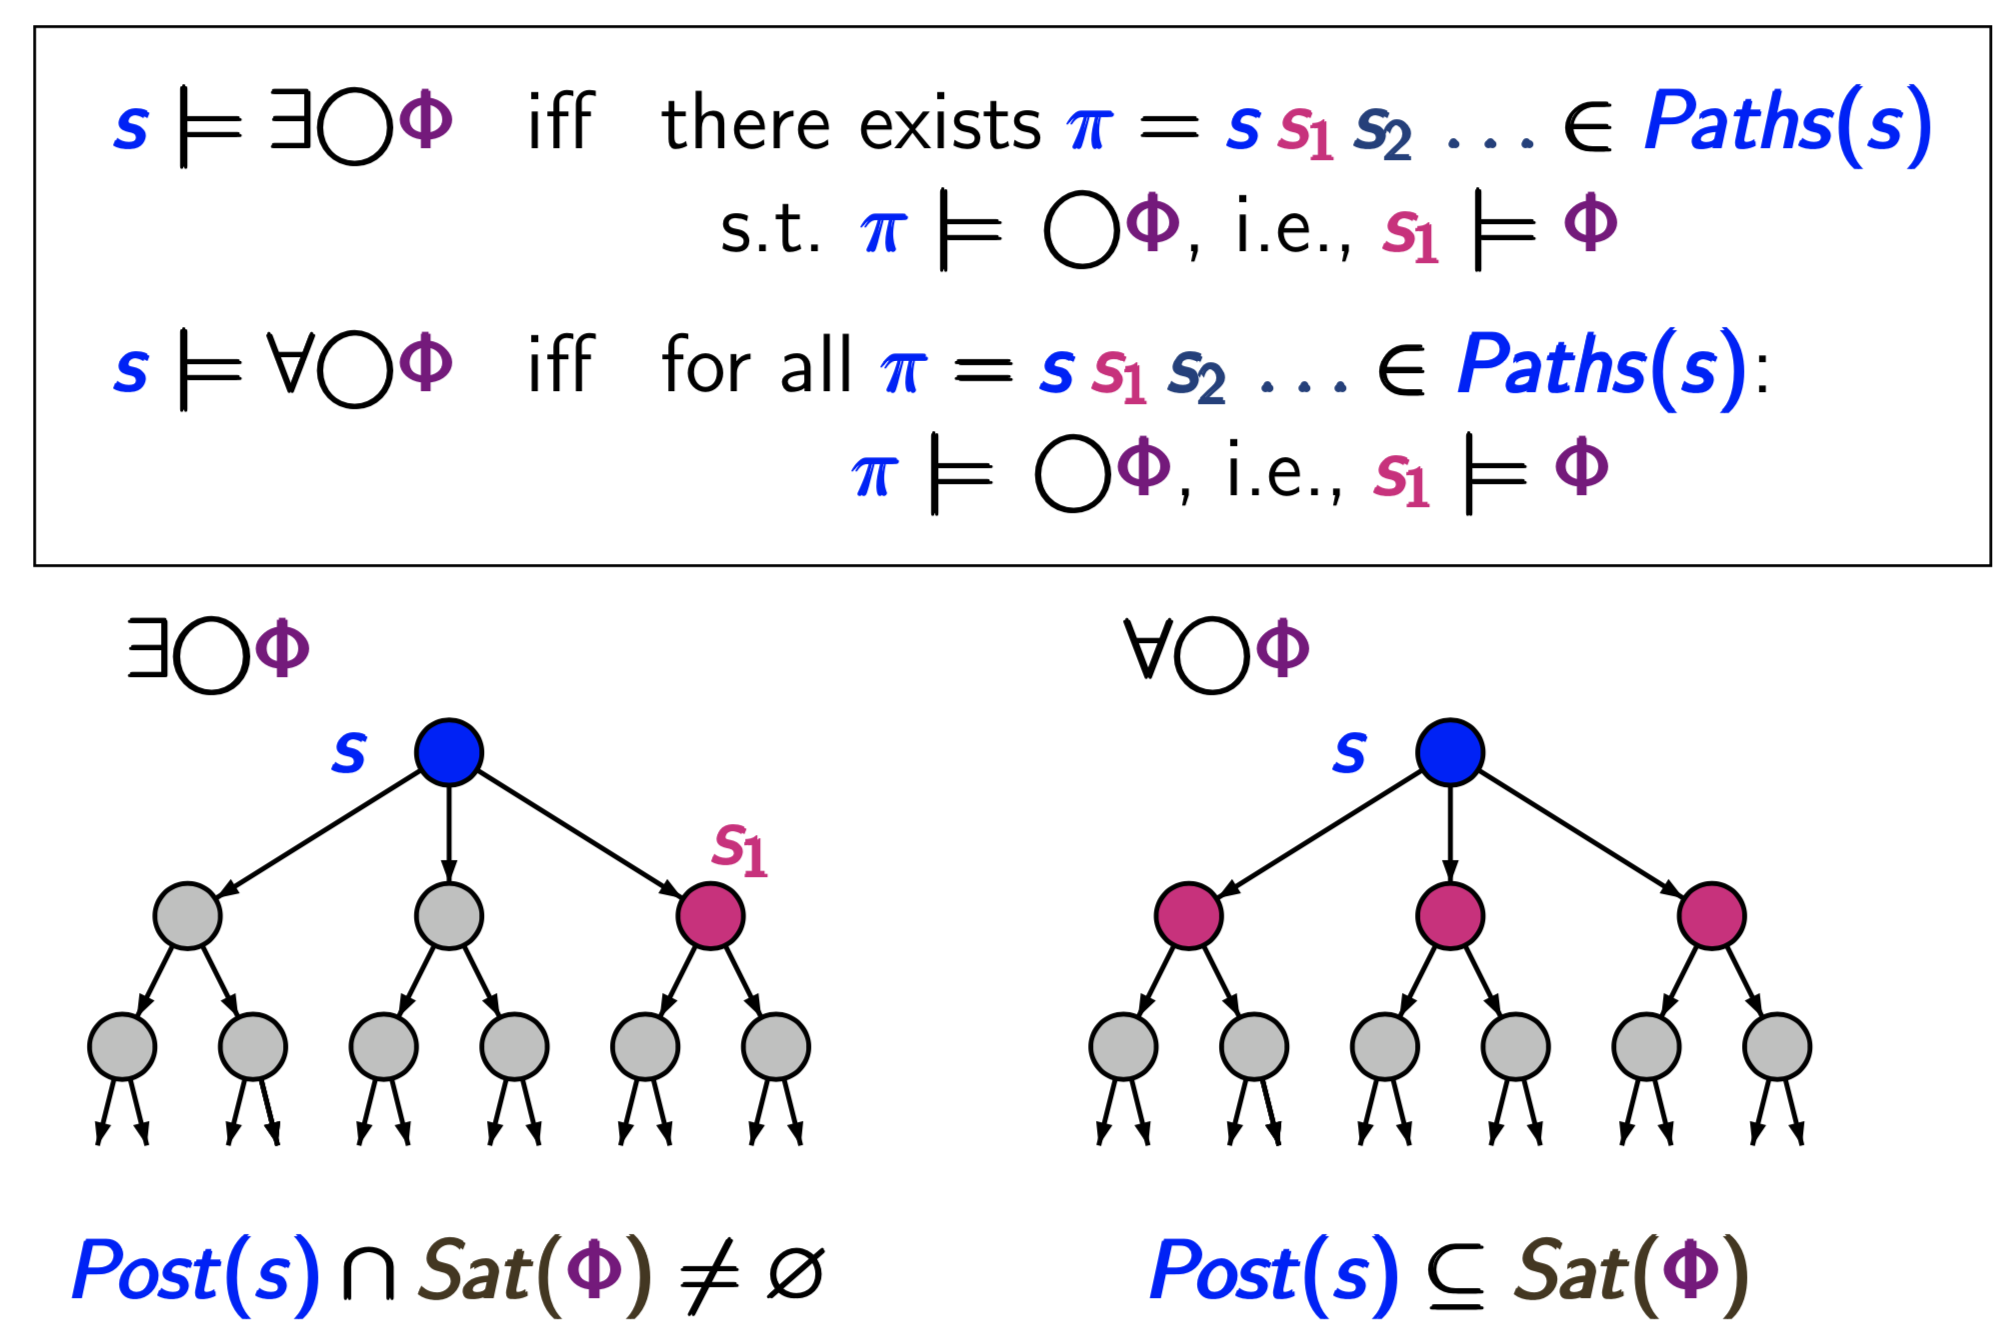
\includegraphics[scale=0.126]{NEXT}
	\end{figure}
\columnbreak
	\begin{figure}[H]
		\centering
		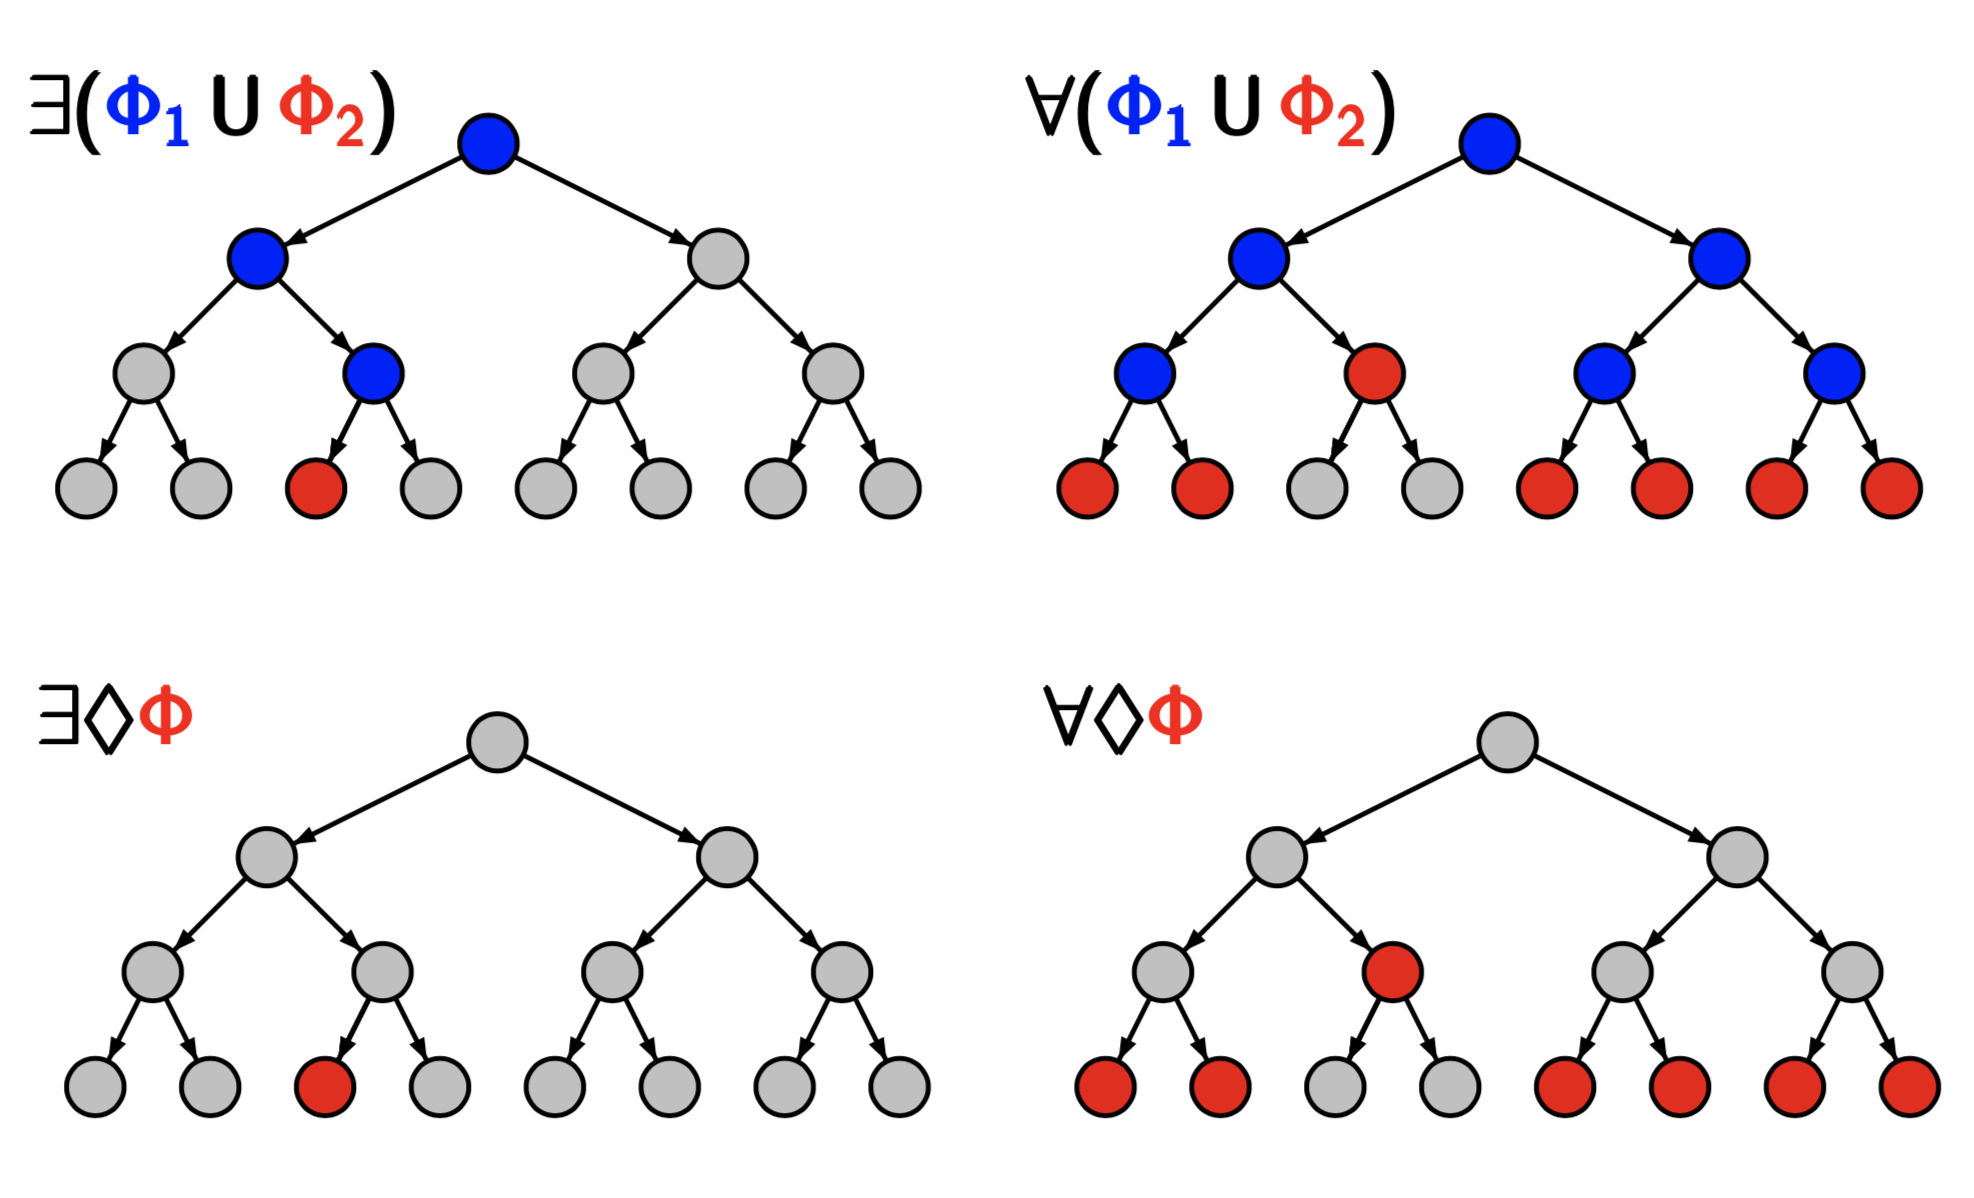
\includegraphics[scale=0.126]{CT1}
	\end{figure}
\columnbreak
	\begin{figure}[H]
		\centering
		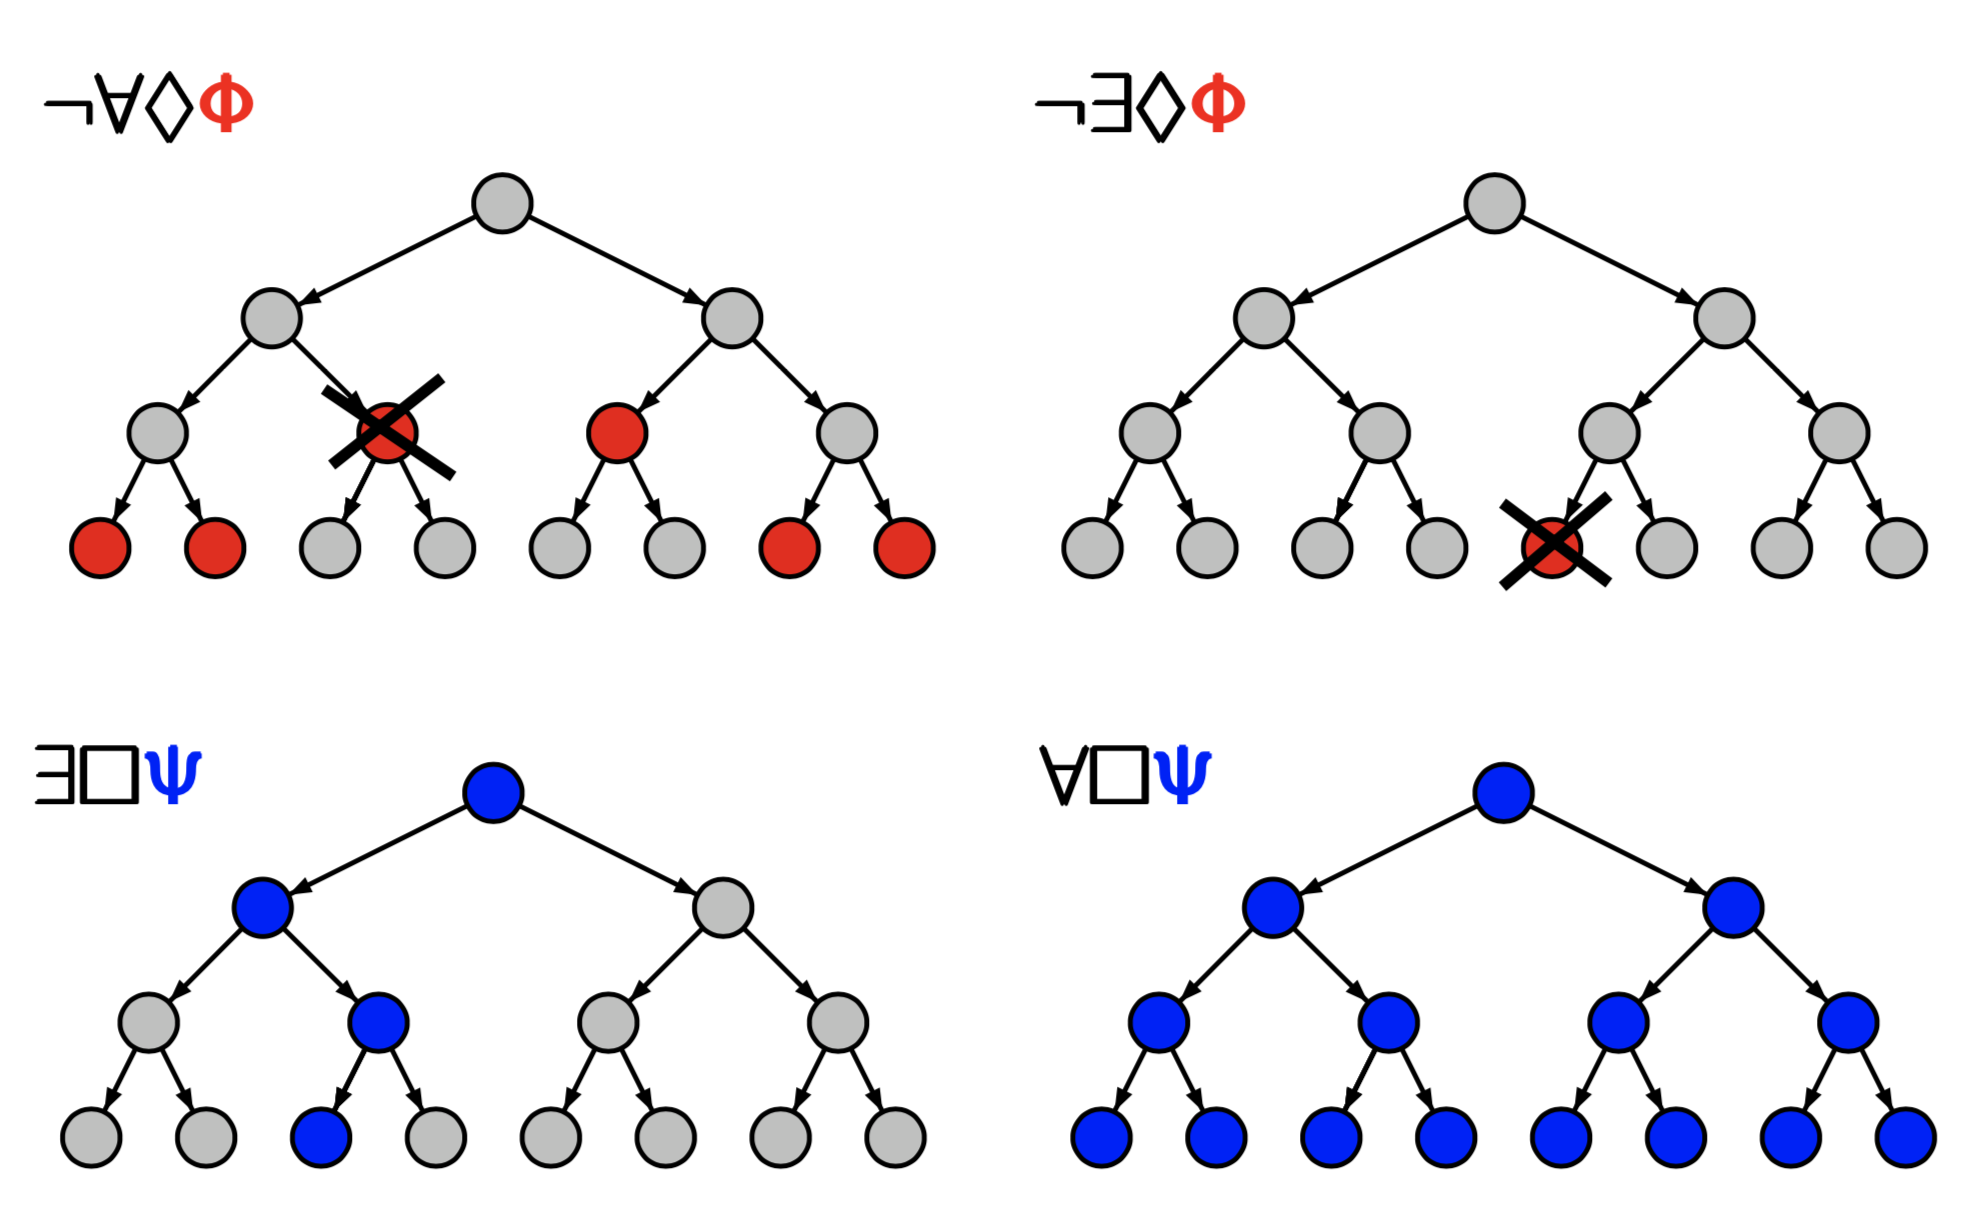
\includegraphics[scale=0.126]{CT2}
	\end{figure}
\end{multicols}

\noindent
Se $\mathcal{T} \nvDash \lnot \phi$, allora \textbf{non} è necessario che $\mathcal{T} \vDash \phi$. Ci sono più stati iniziali (la regola deve essere verificata $\forall s_0$).
\begin{multicols}{2}
	\noindent
\textit{\textbf{Equivalenza tra formule CTL}}.\\
$\phi_1 \equiv \phi_2$ sse, per ogni TS $\mathcal{T}: \mathcal{T} \vDash \phi_1 \Leftrightarrow \mathcal{T} \vDash \phi_2$\\e vale $Sat(\phi_1) = Sat(\phi_2)$.\\\\
$\exists \Diamond (a \land b) \neq \exists \Diamond a \land \exists \Diamond b$\\
$\forall \Diamond (a \land b) \neq \forall \Diamond a \land \forall \Diamond b$\\
$\forall \Box (\phi_1 \land \phi_2) \equiv \forall \Box \phi_1 \land \forall \Box \phi_2$\\
$\exists \Diamond (\phi_1 \lor \phi_2) \equiv \exists \Diamond \phi_1 \lor \exists \Diamond \phi_2$
\columnbreak

\noindent
\textit{\textbf{Duality laws}}.\\
$\forall \Box \phi \equiv \lnot \exists \Diamond \lnot \phi$\\
$\forall \Diamond \phi \equiv \lnot \exists \Box \lnot \phi$\\
$\forall \bigcirc \phi \equiv \lnot \exists \bigcirc \lnot \phi$\\
$\exists \bigcirc \phi \equiv \lnot \forall \bigcirc \lnot \phi$\\
$\forall(\phi \bigcup \psi) \equiv \lnot \exists ((\lnot \psi) \bigcup (\lnot \phi \land \lnot \psi)) \land \lnot \exists \Box \lnot \psi$\\
\\
$\forall \bigcup$ e $\forall \bigcirc$ sono esprimibili attraverso $\exists \bigcup$, $\exists \bigcirc$ e $\exists \Box$
\end{multicols}


\section*{Equivalenza tra formule LTL e CTL}
\addcontentsline{toc}{section}{Equivalenza tra formule LTL e CTL}
Sia $\phi$ una formula CTL e $\psi$ una formula LTL: $\phi \equiv \psi$ sse $\forall \mathcal{T}$ e $\forall s \in \mathcal{T}$: ~$s \vDash_{CTL} \phi ~\Leftrightarrow~ s \vDash_{LTL} \psi$
\begin{multicols}{2}
	\begin{figure}[H]
		\centering
		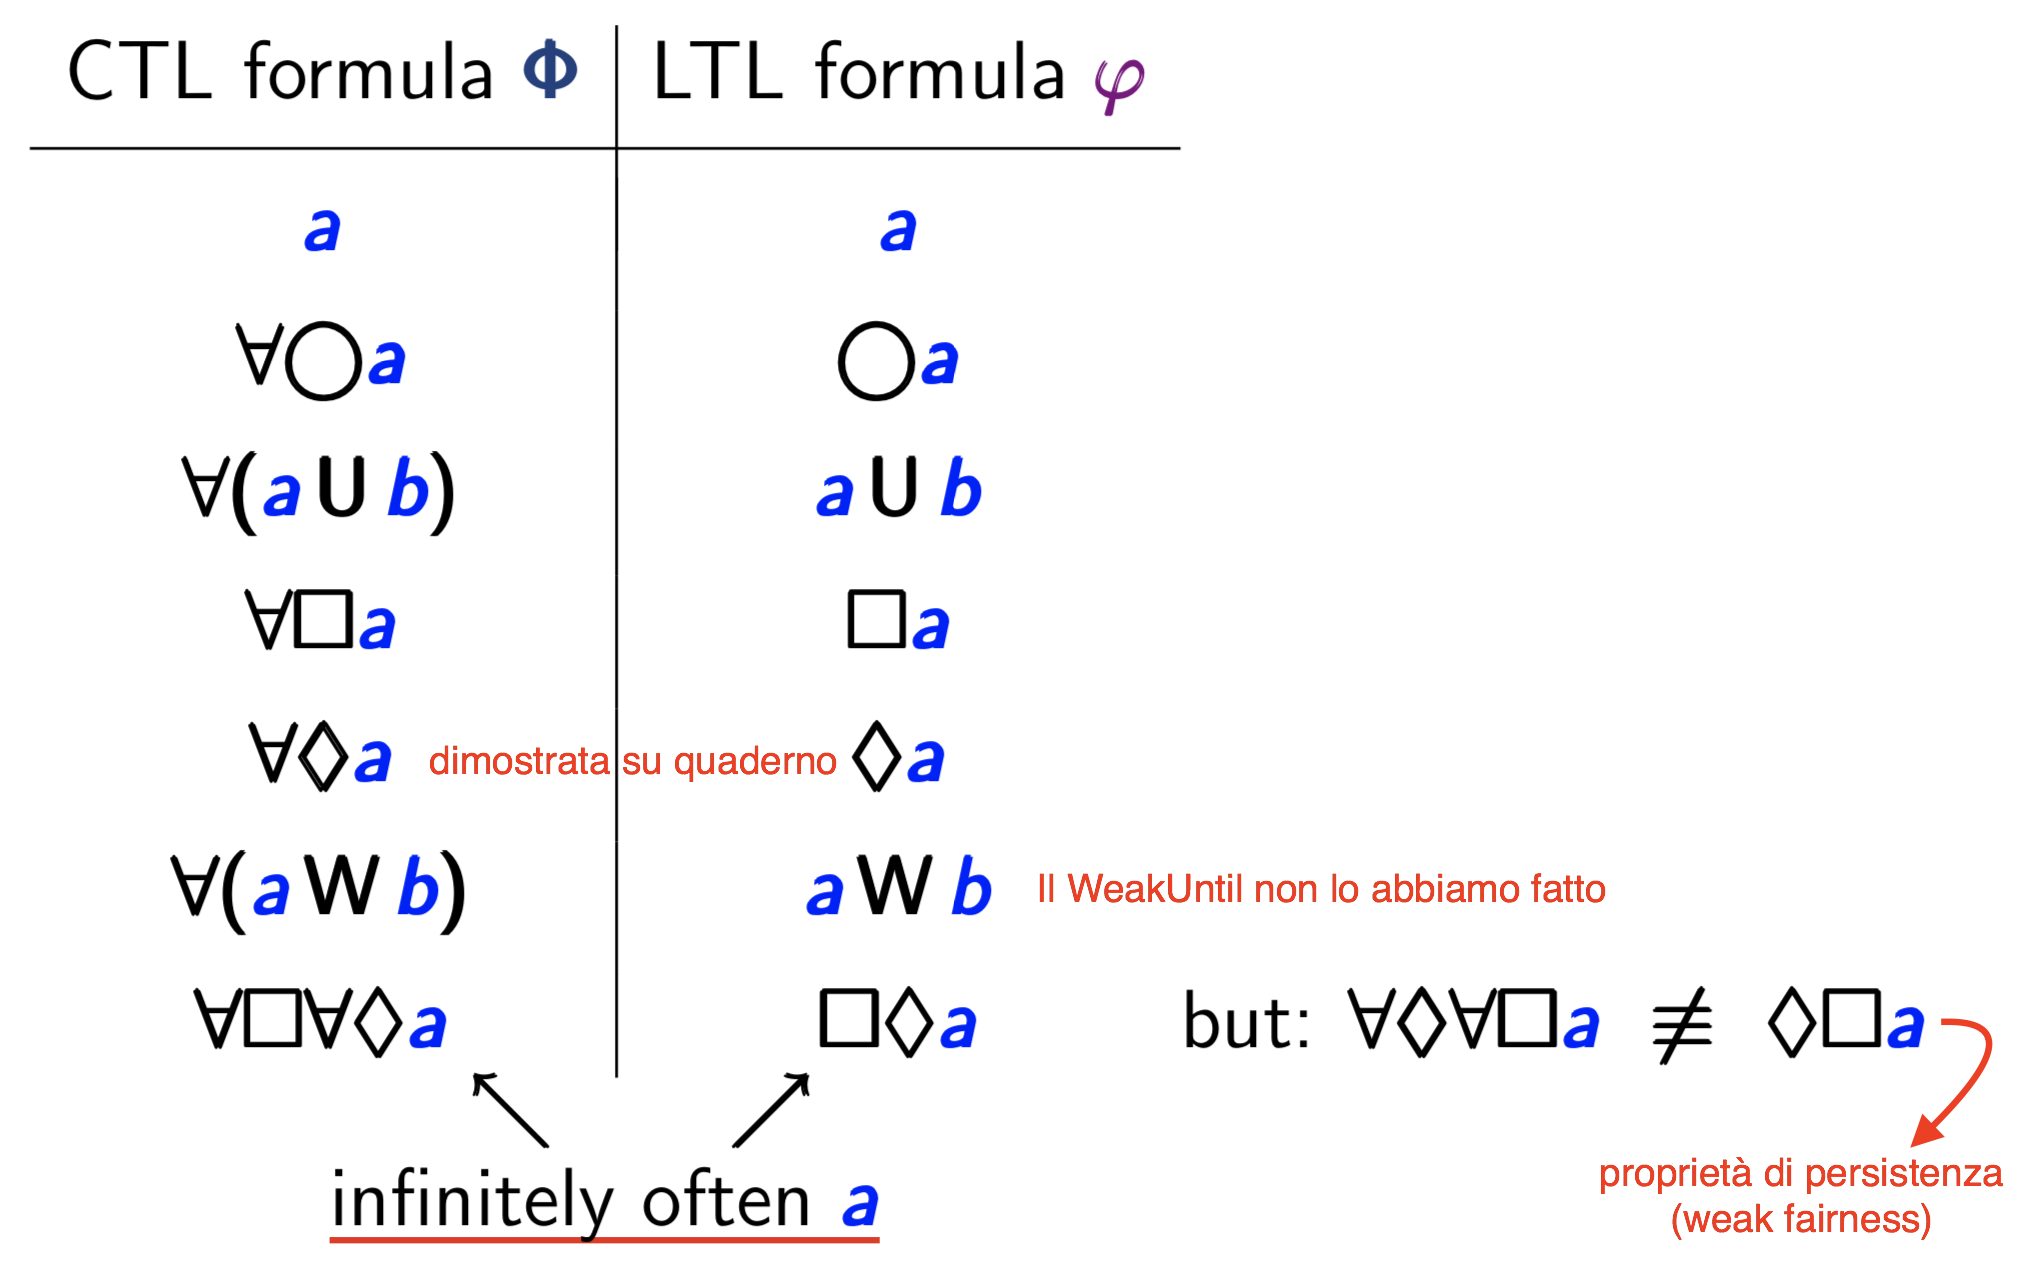
\includegraphics[scale=0.2]{CTLvLTL}
	\end{figure}
\columnbreak
	\noindent
	\textit{\textbf{Dimostrazione: in CTL non vale weak fairness}}\\
	$\Diamond \Box a \neq \forall \Diamond \forall \Box a$\\
	Nessuna formula LTL è equivalente a $\forall \Diamond \forall \Box a$
	\begin{figure}[H]
		\centering
		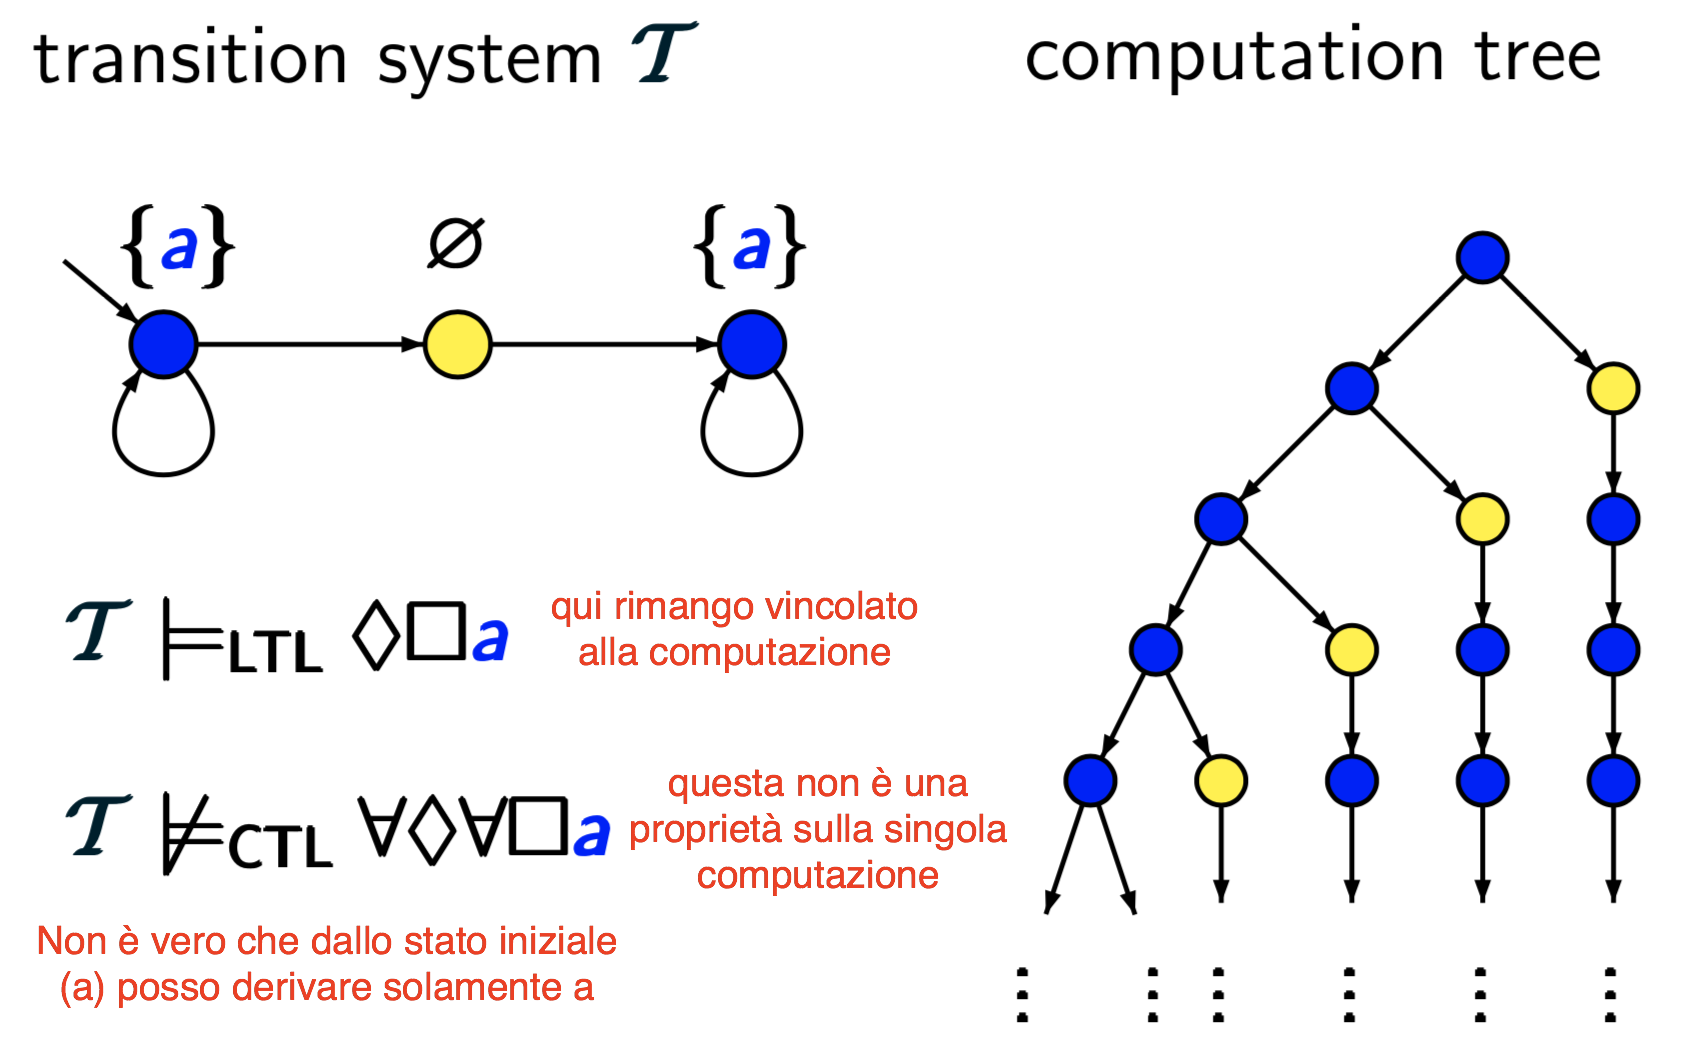
\includegraphics[scale=0.16]{vs1}
	\end{figure}
\end{multicols}
\hrule
\begin{multicols}{2}
	\noindent
	$\Diamond (a \land \bigcirc a) \neq \forall \Diamond (a \land \forall \bigcirc a)$
	\begin{figure}[H]
		\centering
		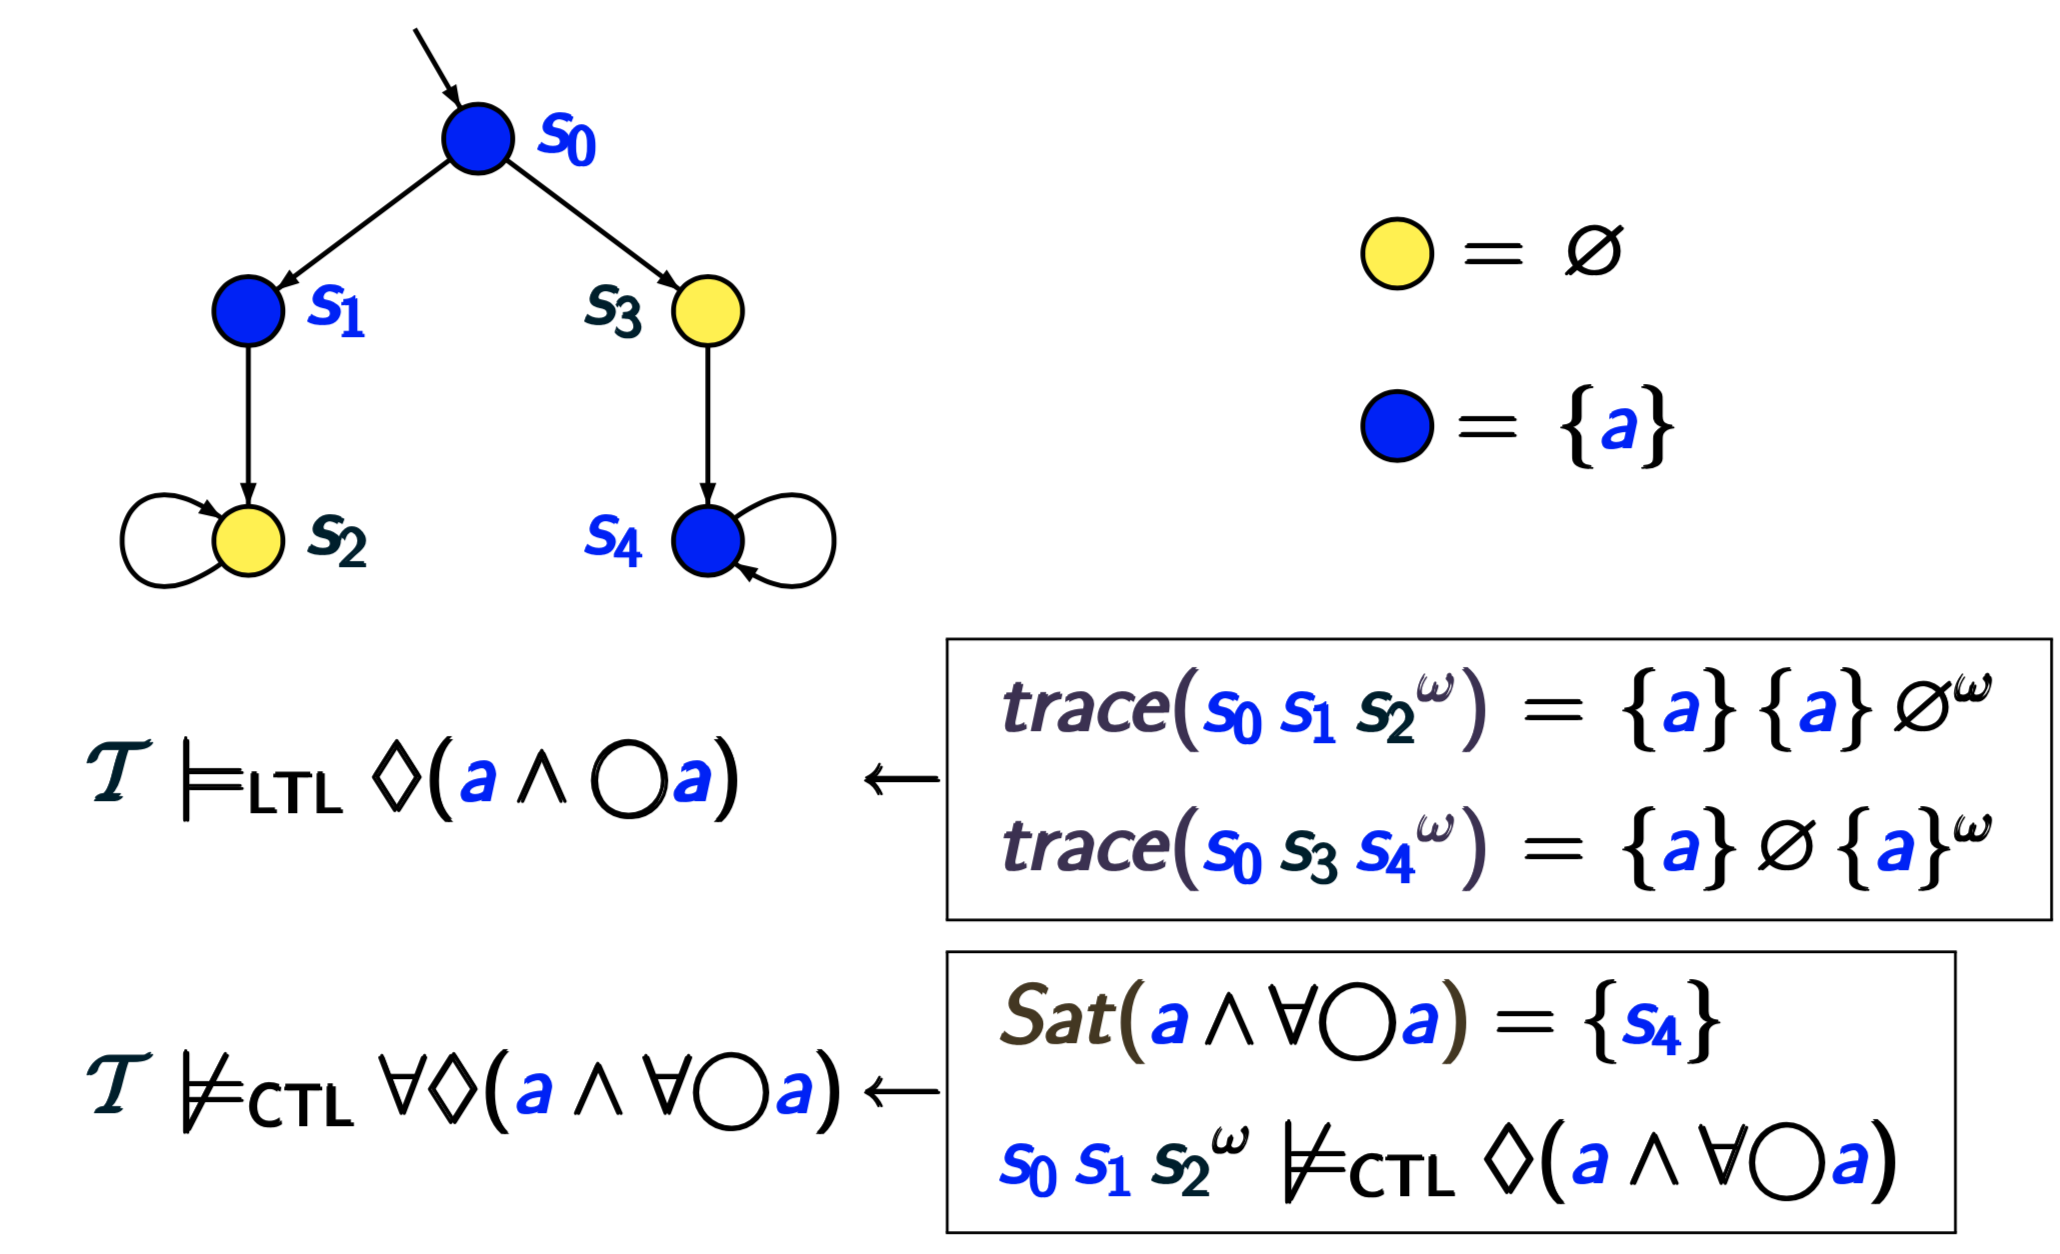
\includegraphics[scale=0.13]{vs2}
	\end{figure}
\columnbreak
\begin{figure}[H]
	\centering
	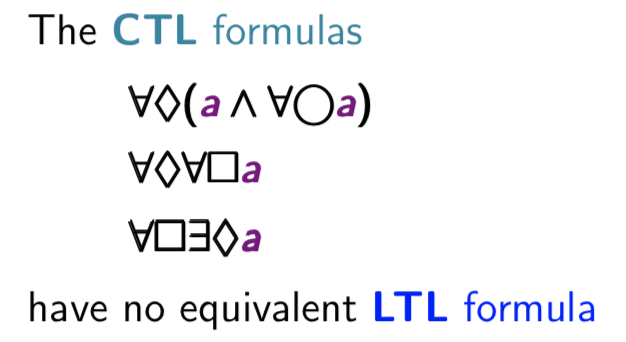
\includegraphics[scale=0.3]{v3}
\end{figure}
\begin{figure}[H]
	\centering
	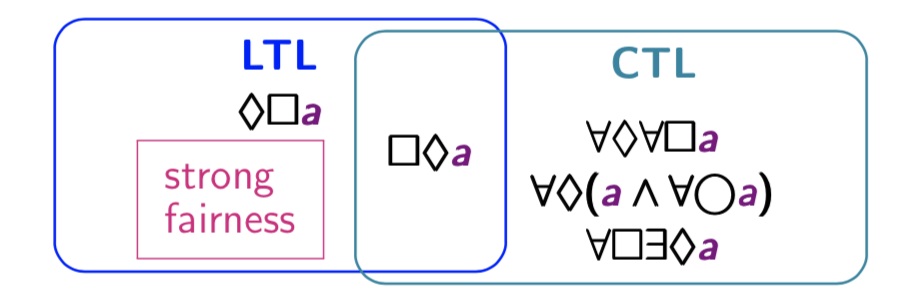
\includegraphics[scale=0.27]{v4}
\end{figure}
\end{multicols}
\hrule
\begin{multicols}{3}
\begin{figure}[H]
	\centering
	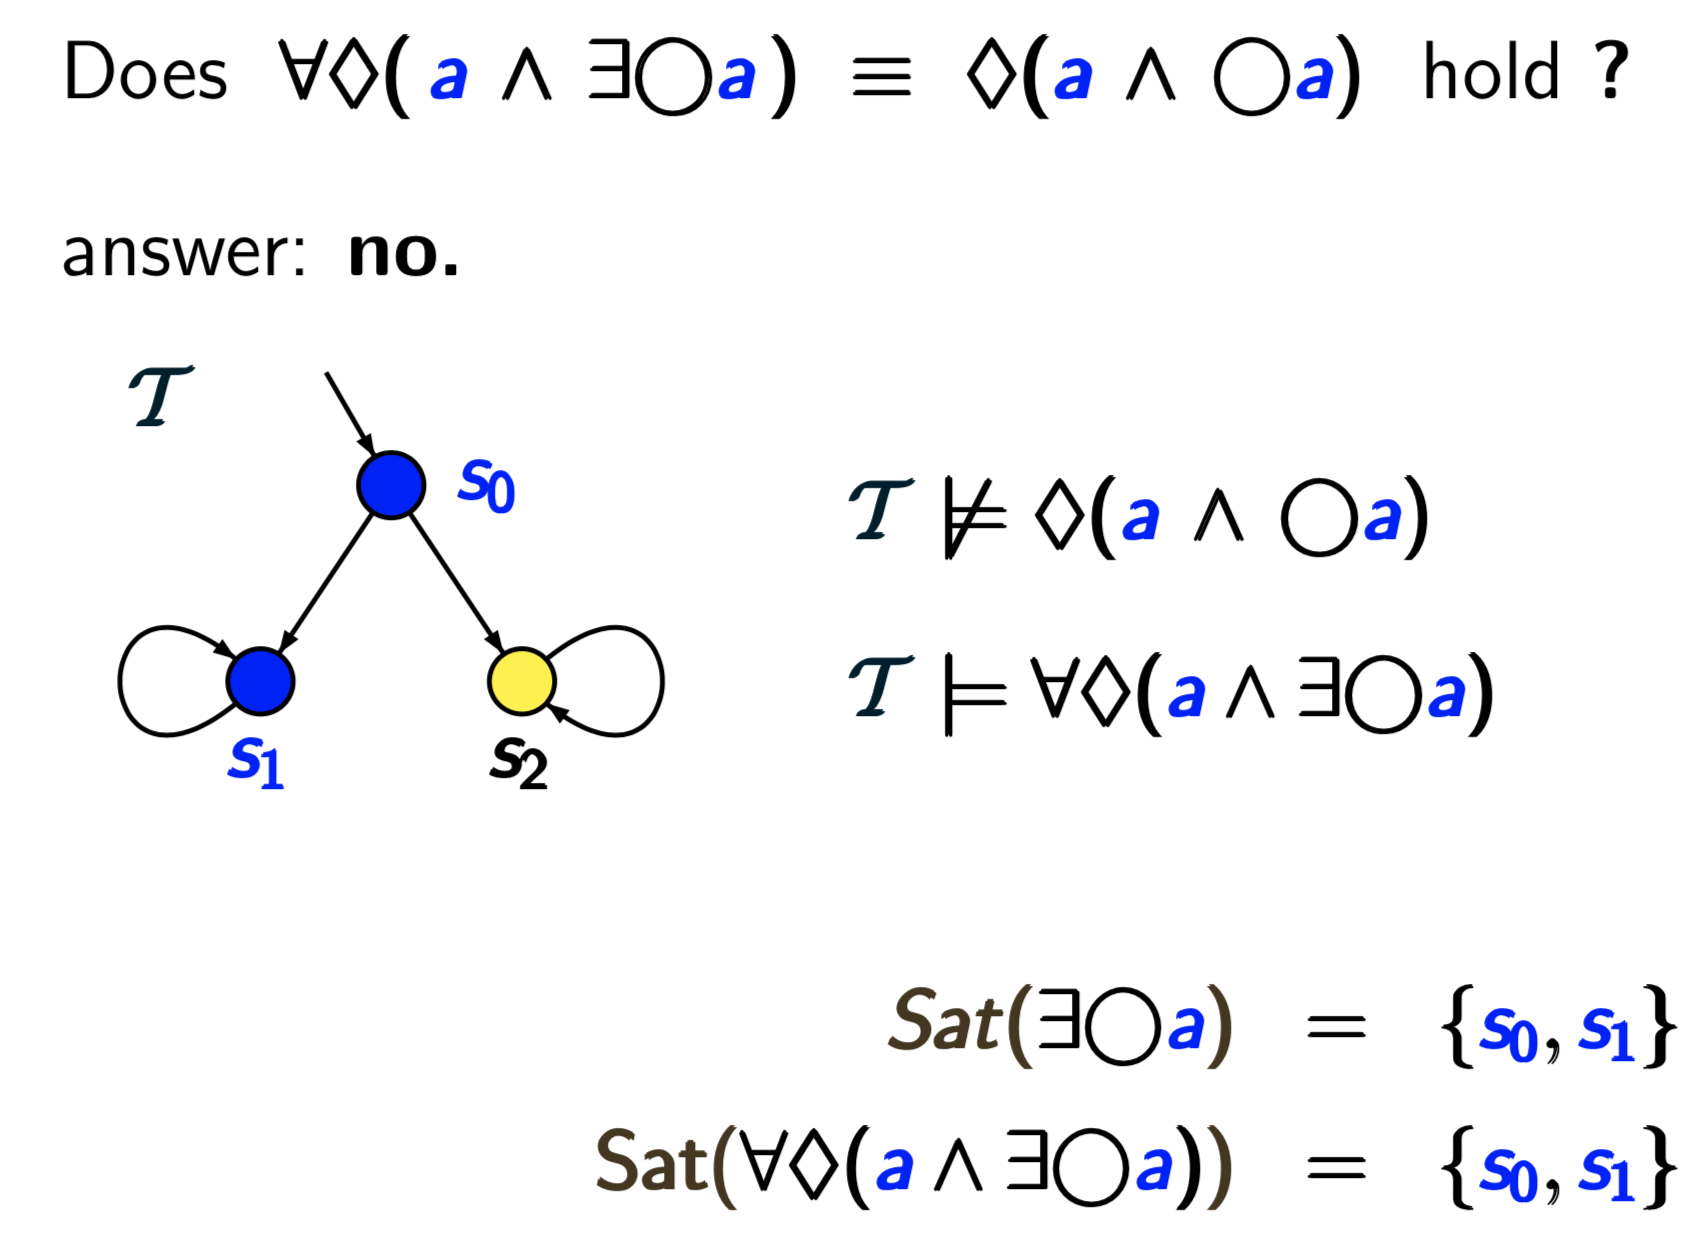
\includegraphics[scale=0.14]{vv}
\end{figure}
\columnbreak
\begin{figure}[H]
	\centering
	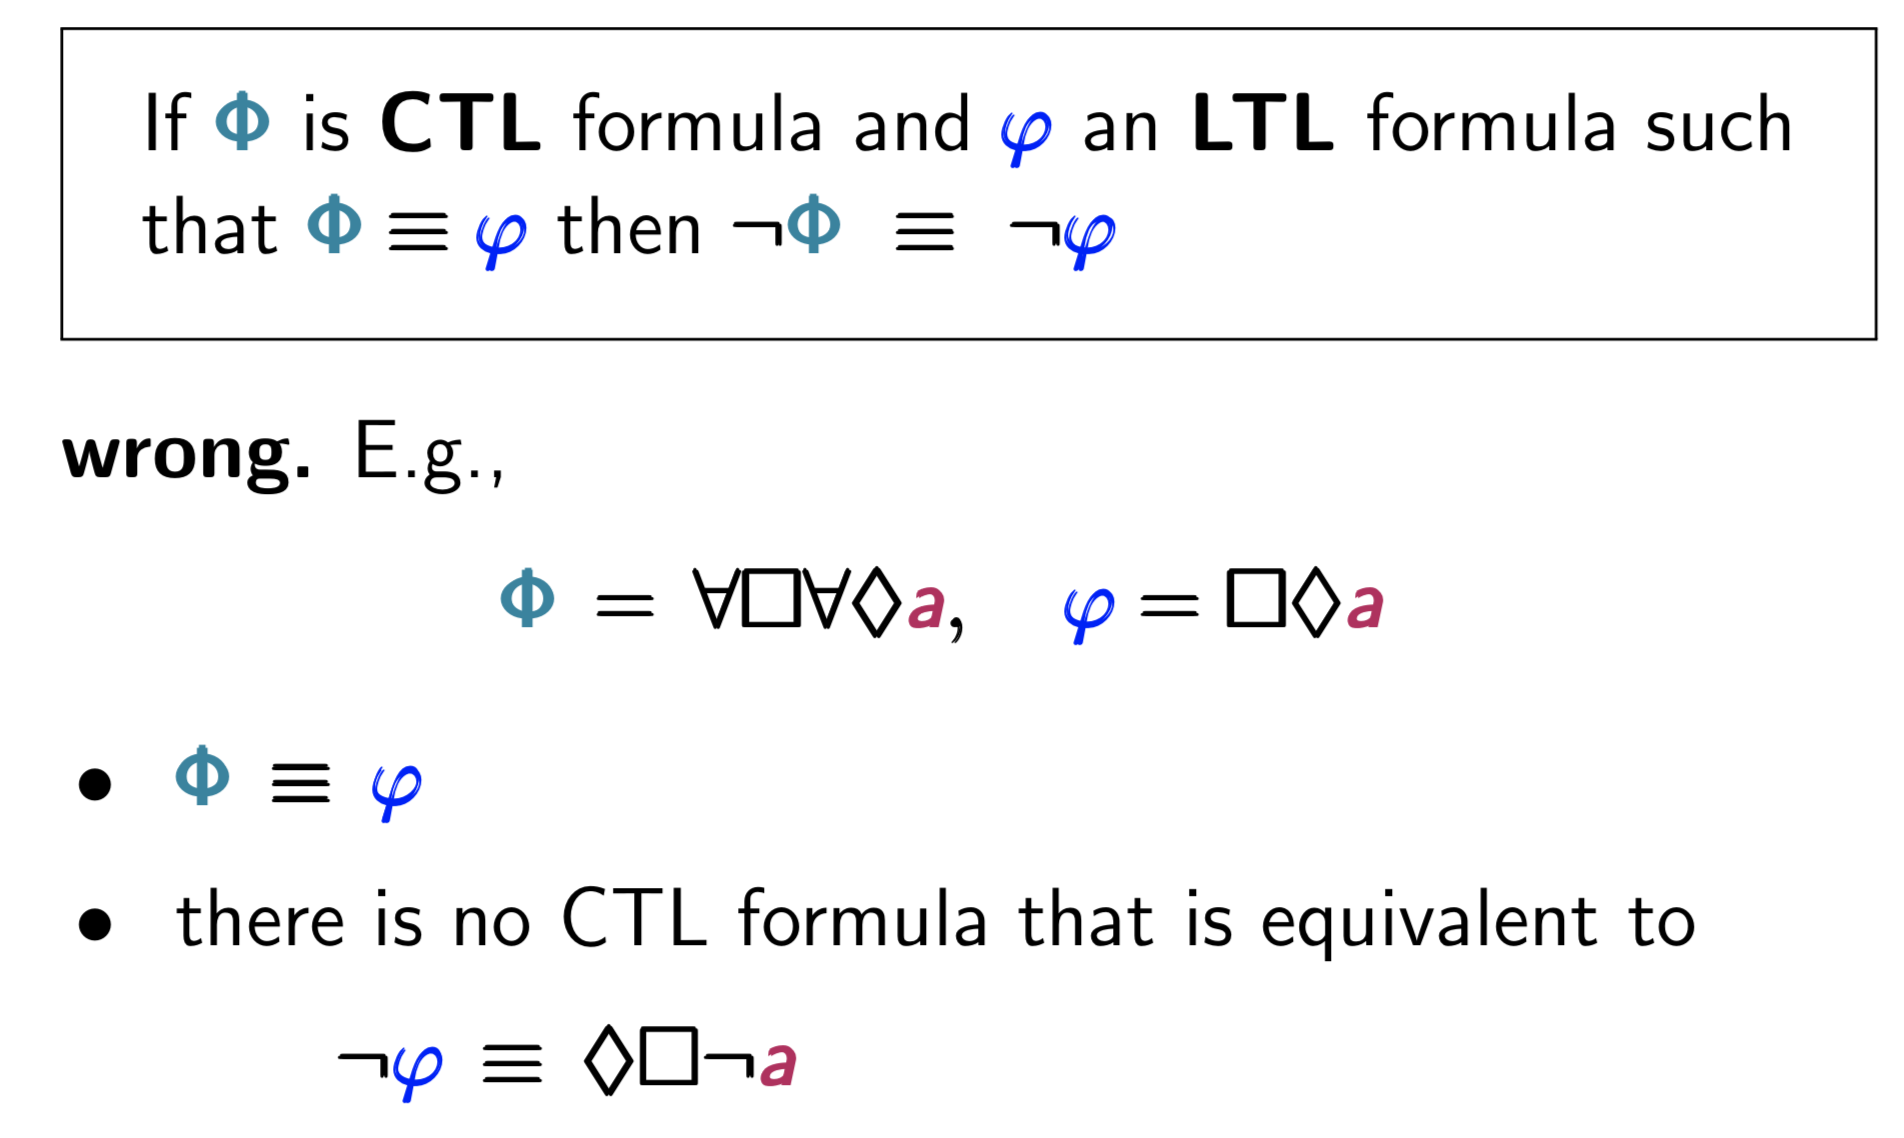
\includegraphics[scale=0.15]{wrong}
\end{figure}
\columnbreak
\noindent
Se $\mathcal{T}_1$ e $\mathcal{T}_2$ sono \textit{trace equivalent} \textbf{NON} è vero che $\mathcal{T}_1 \vDash \phi$ sse $\mathcal{T}_2 \vDash \phi$.
\begin{figure}[H]
	\centering
	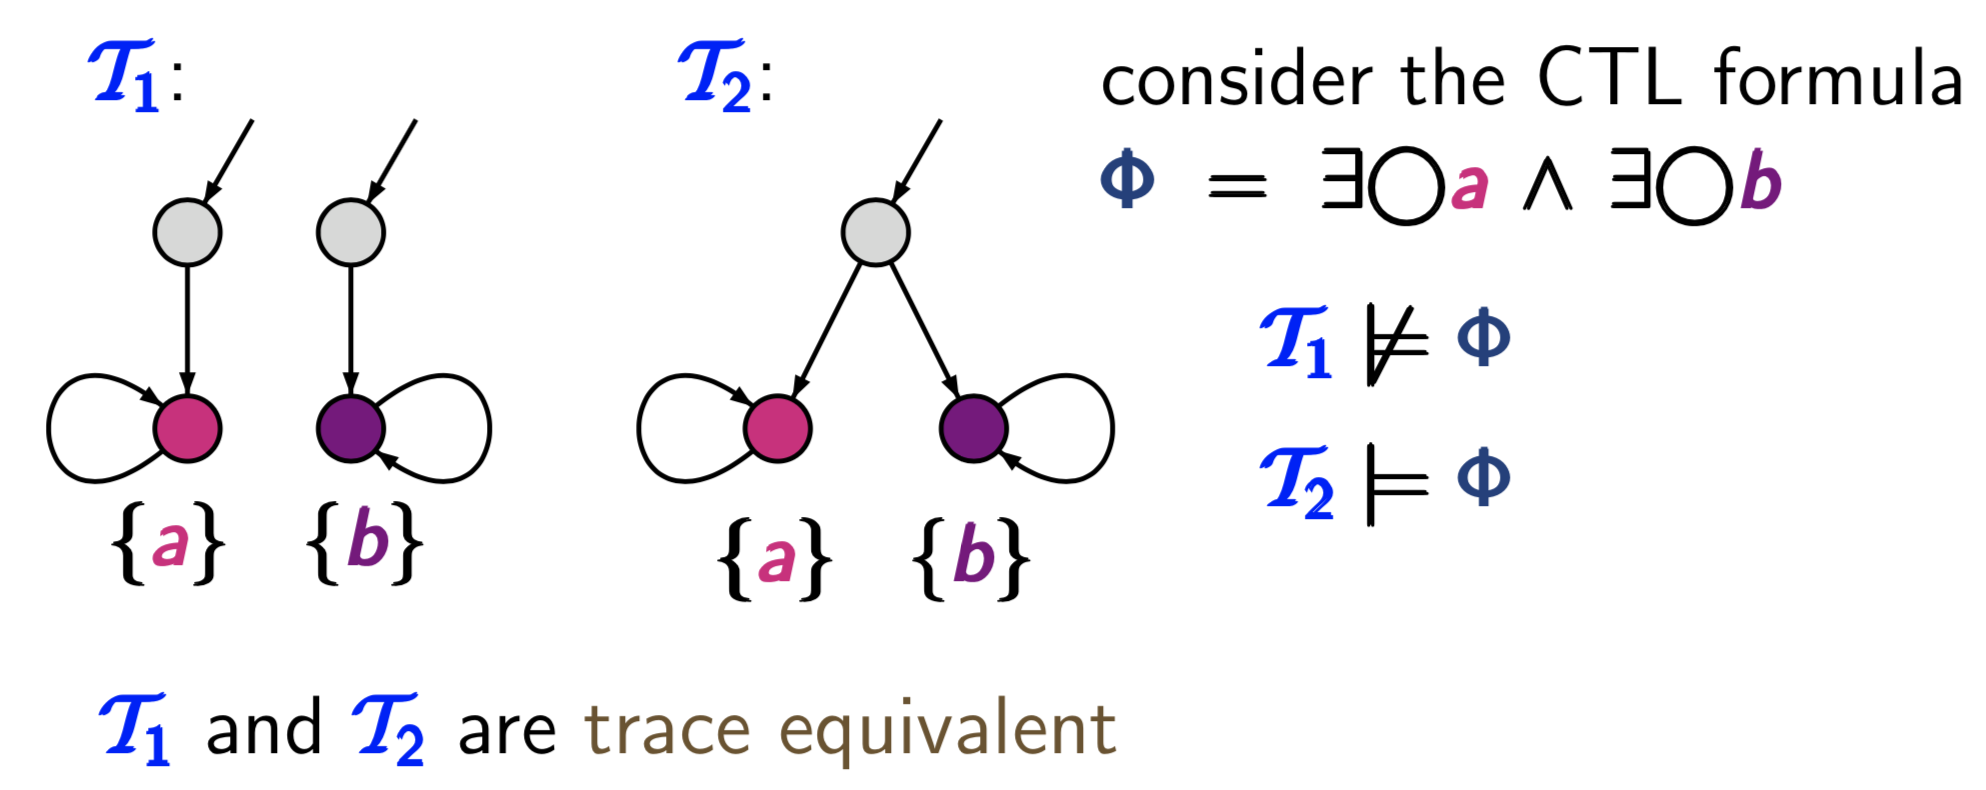
\includegraphics[scale=0.12]{end}
\end{figure}
\end{multicols}


\section*{CTL*}
\addcontentsline{toc}{section}{CTL*}
\begin{multicols}{3}
\begin{figure}[H]
	\centering
	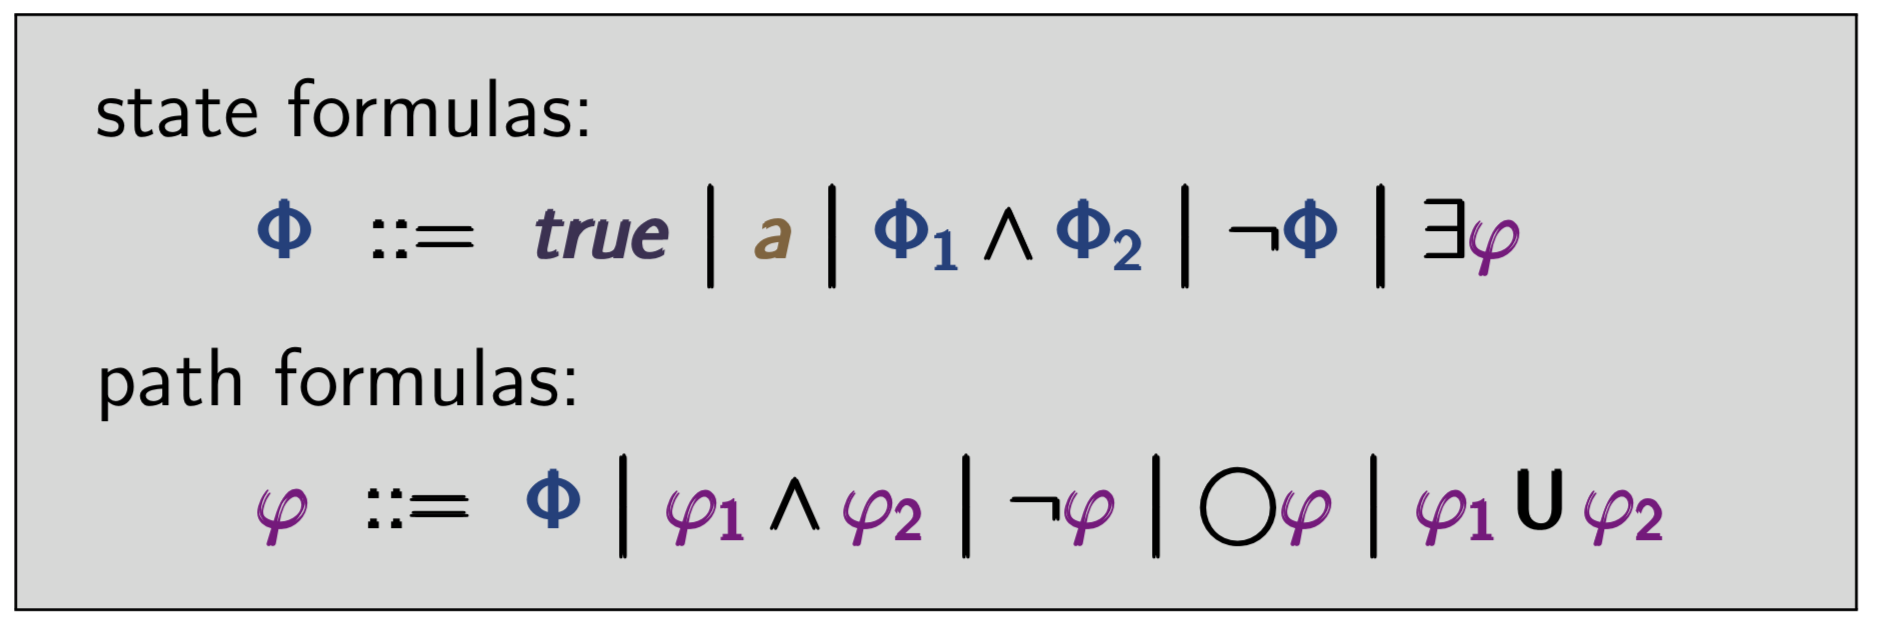
\includegraphics[scale=0.15]{CTL*}
\end{figure}
\noindent
Con CTL* è possibile scrivere la proprietà di Liveness.
\columnbreak
\begin{figure}[H]
	\centering
	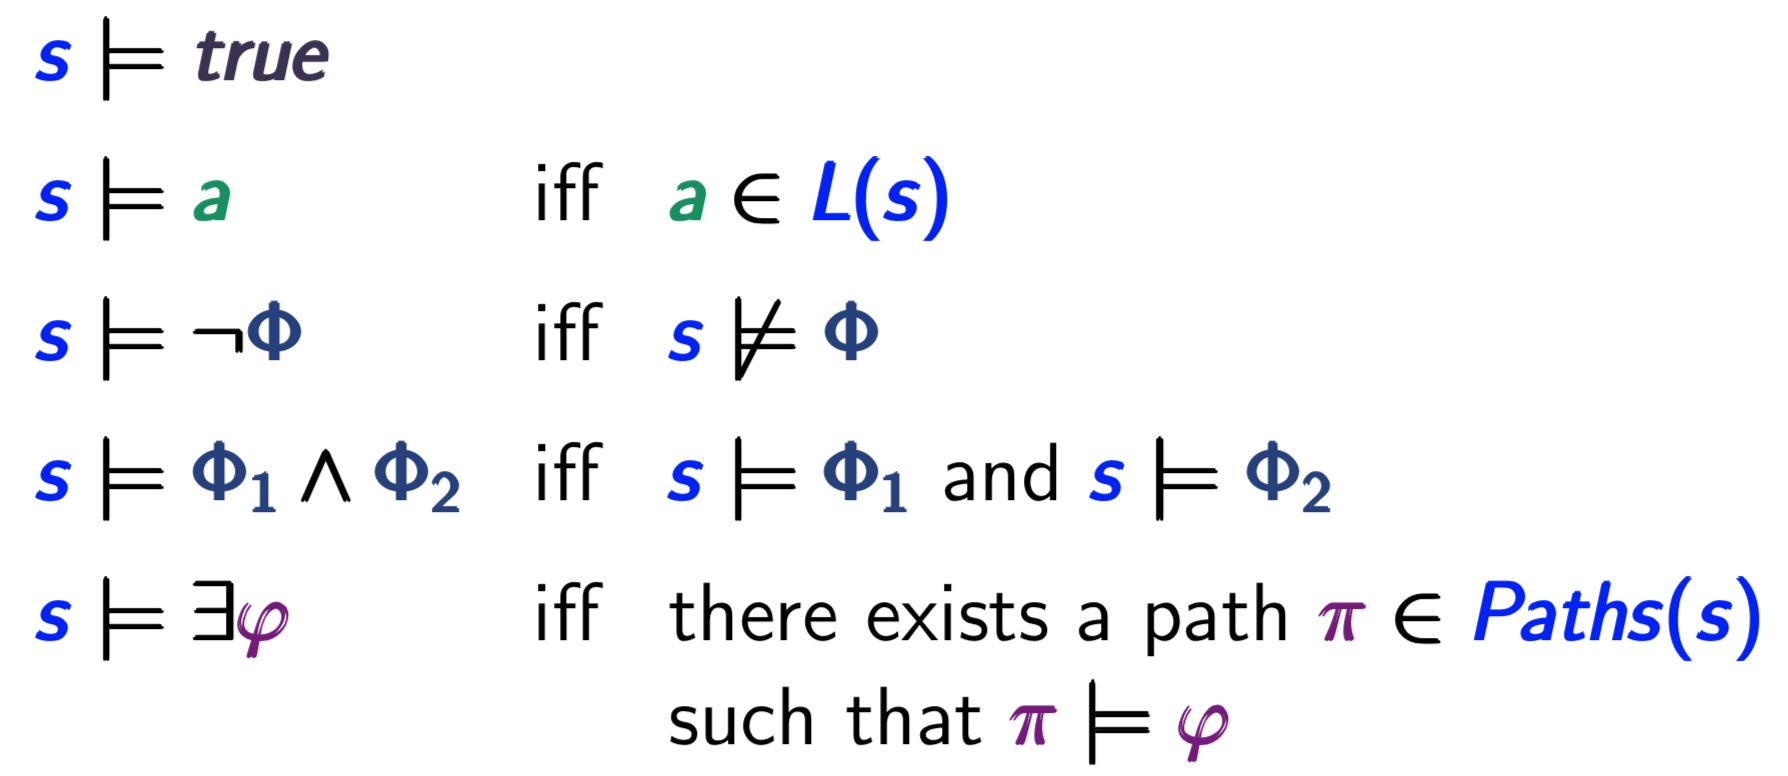
\includegraphics[scale=0.15]{STATECTL*}
\end{figure}
\columnbreak
\begin{figure}[H]
	\centering
	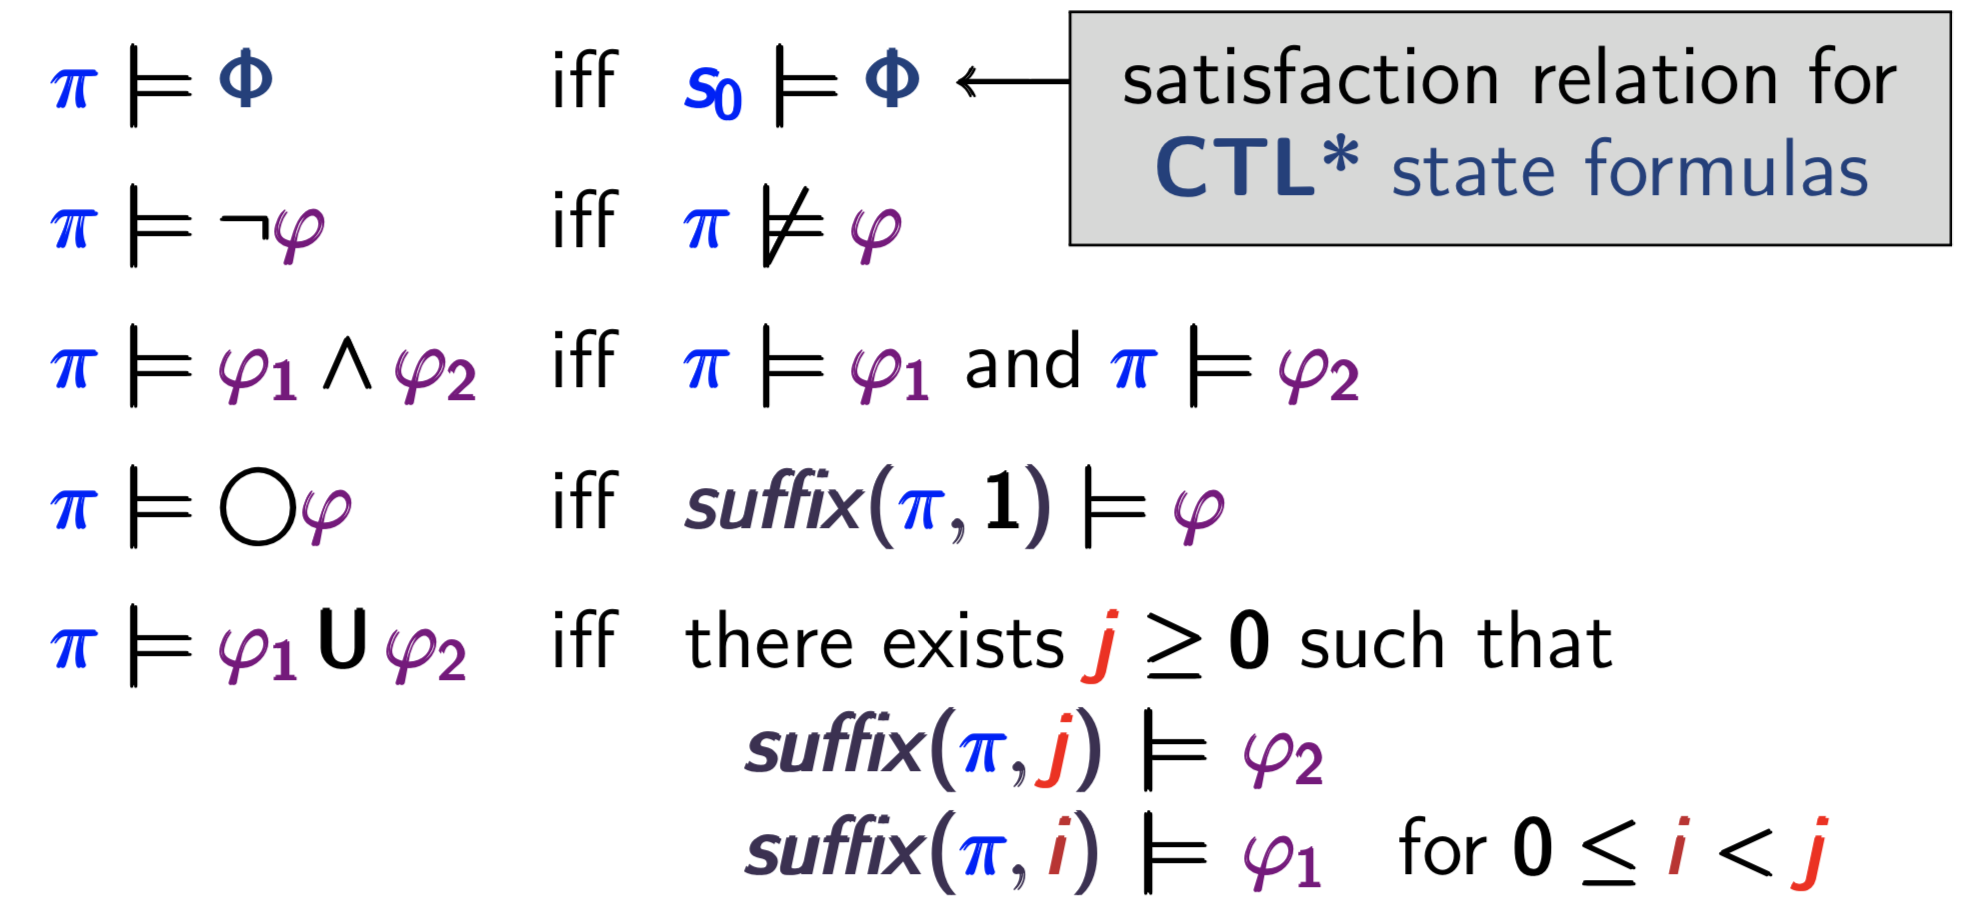
\includegraphics[scale=0.15]{PATHCTL*}
\end{figure}
\end{multicols}
\hrule
\begin{multicols}{3}
	\begin{figure}[H]
		\centering
		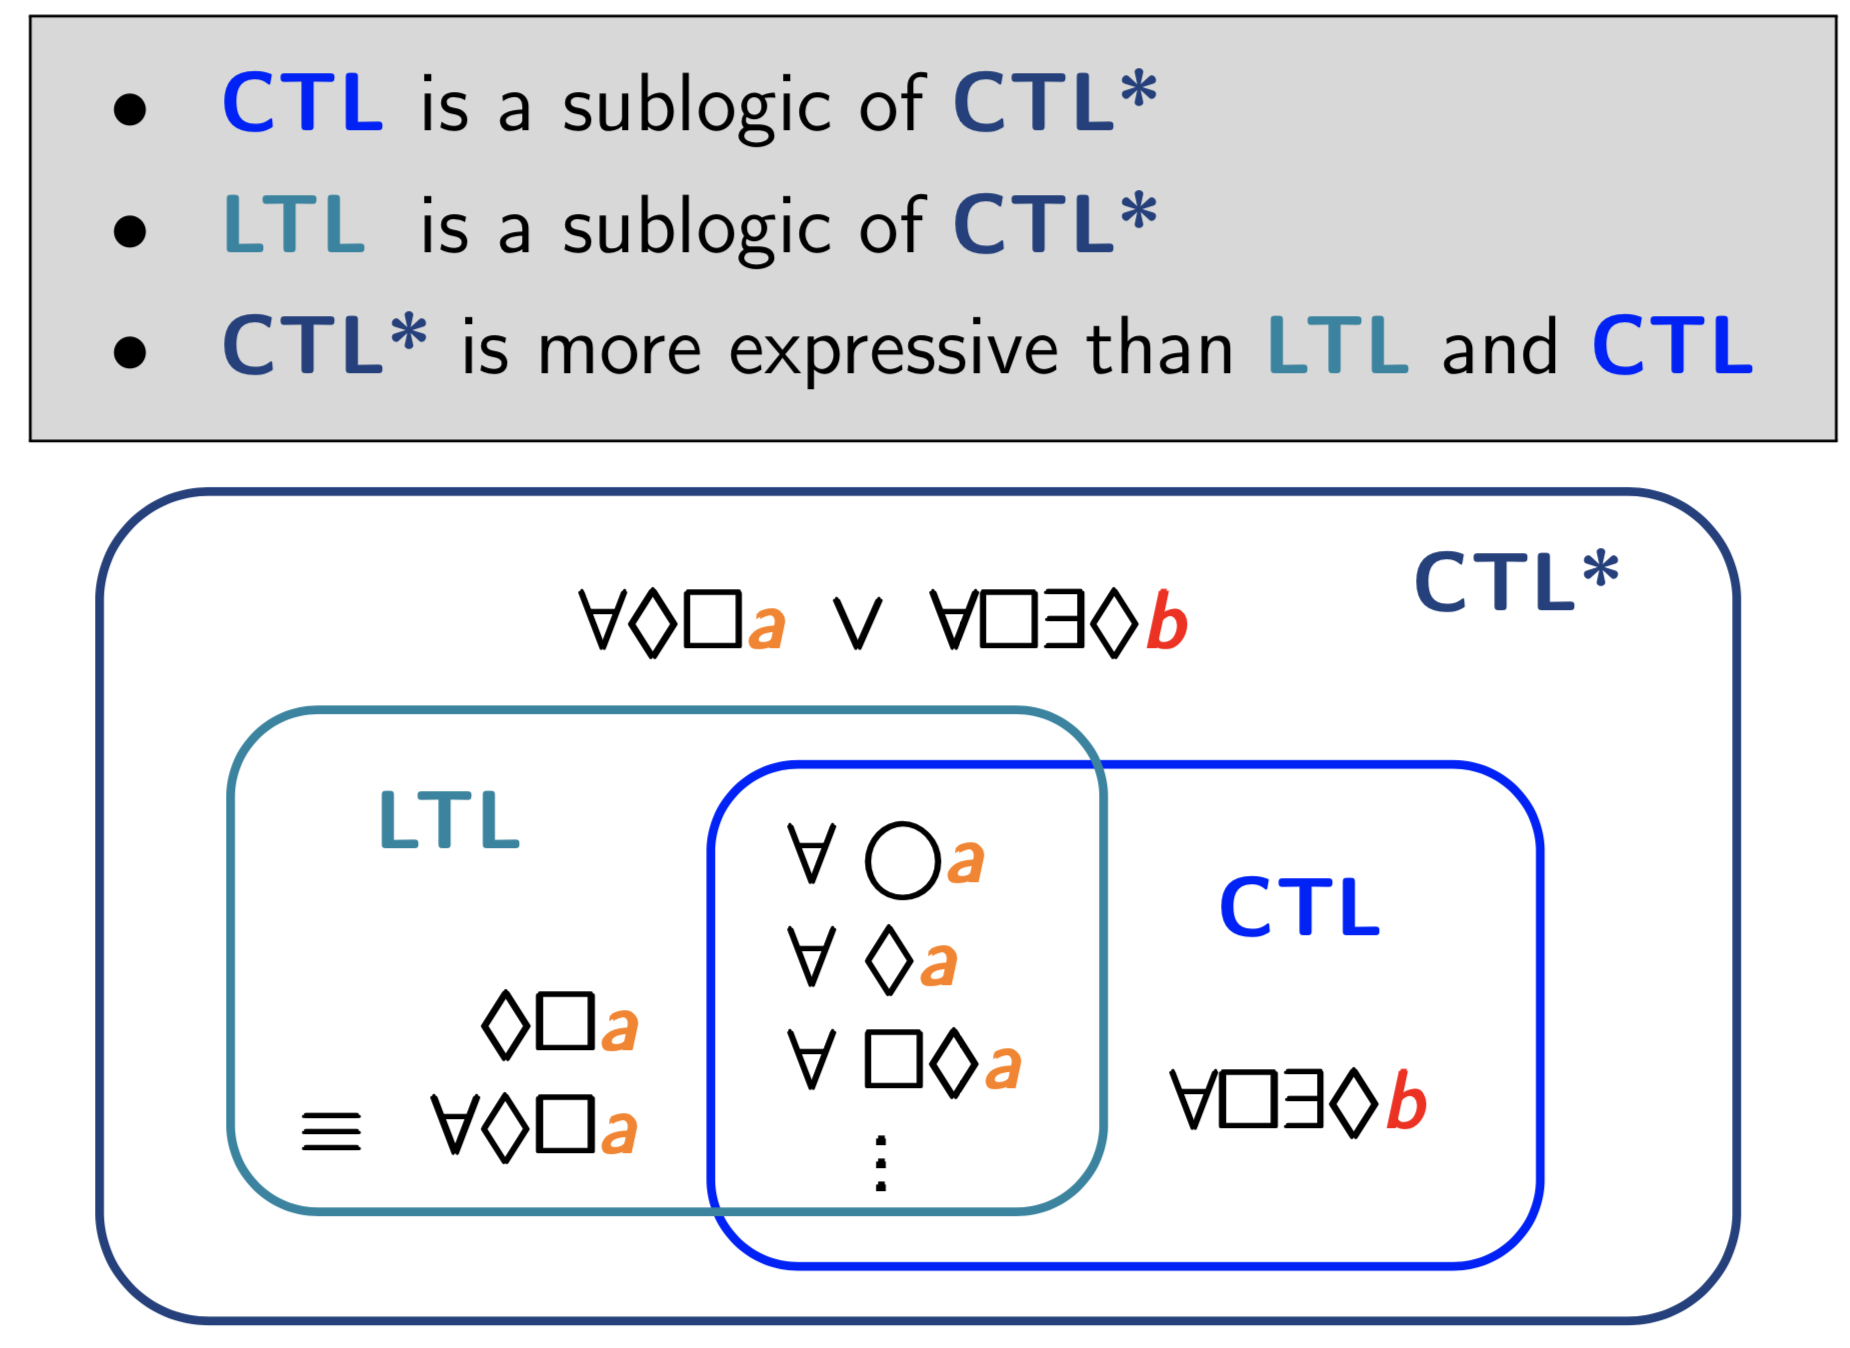
\includegraphics[scale=0.15]{*3}
	\end{figure}
	\columnbreak
	\begin{figure}[H]
		\centering
		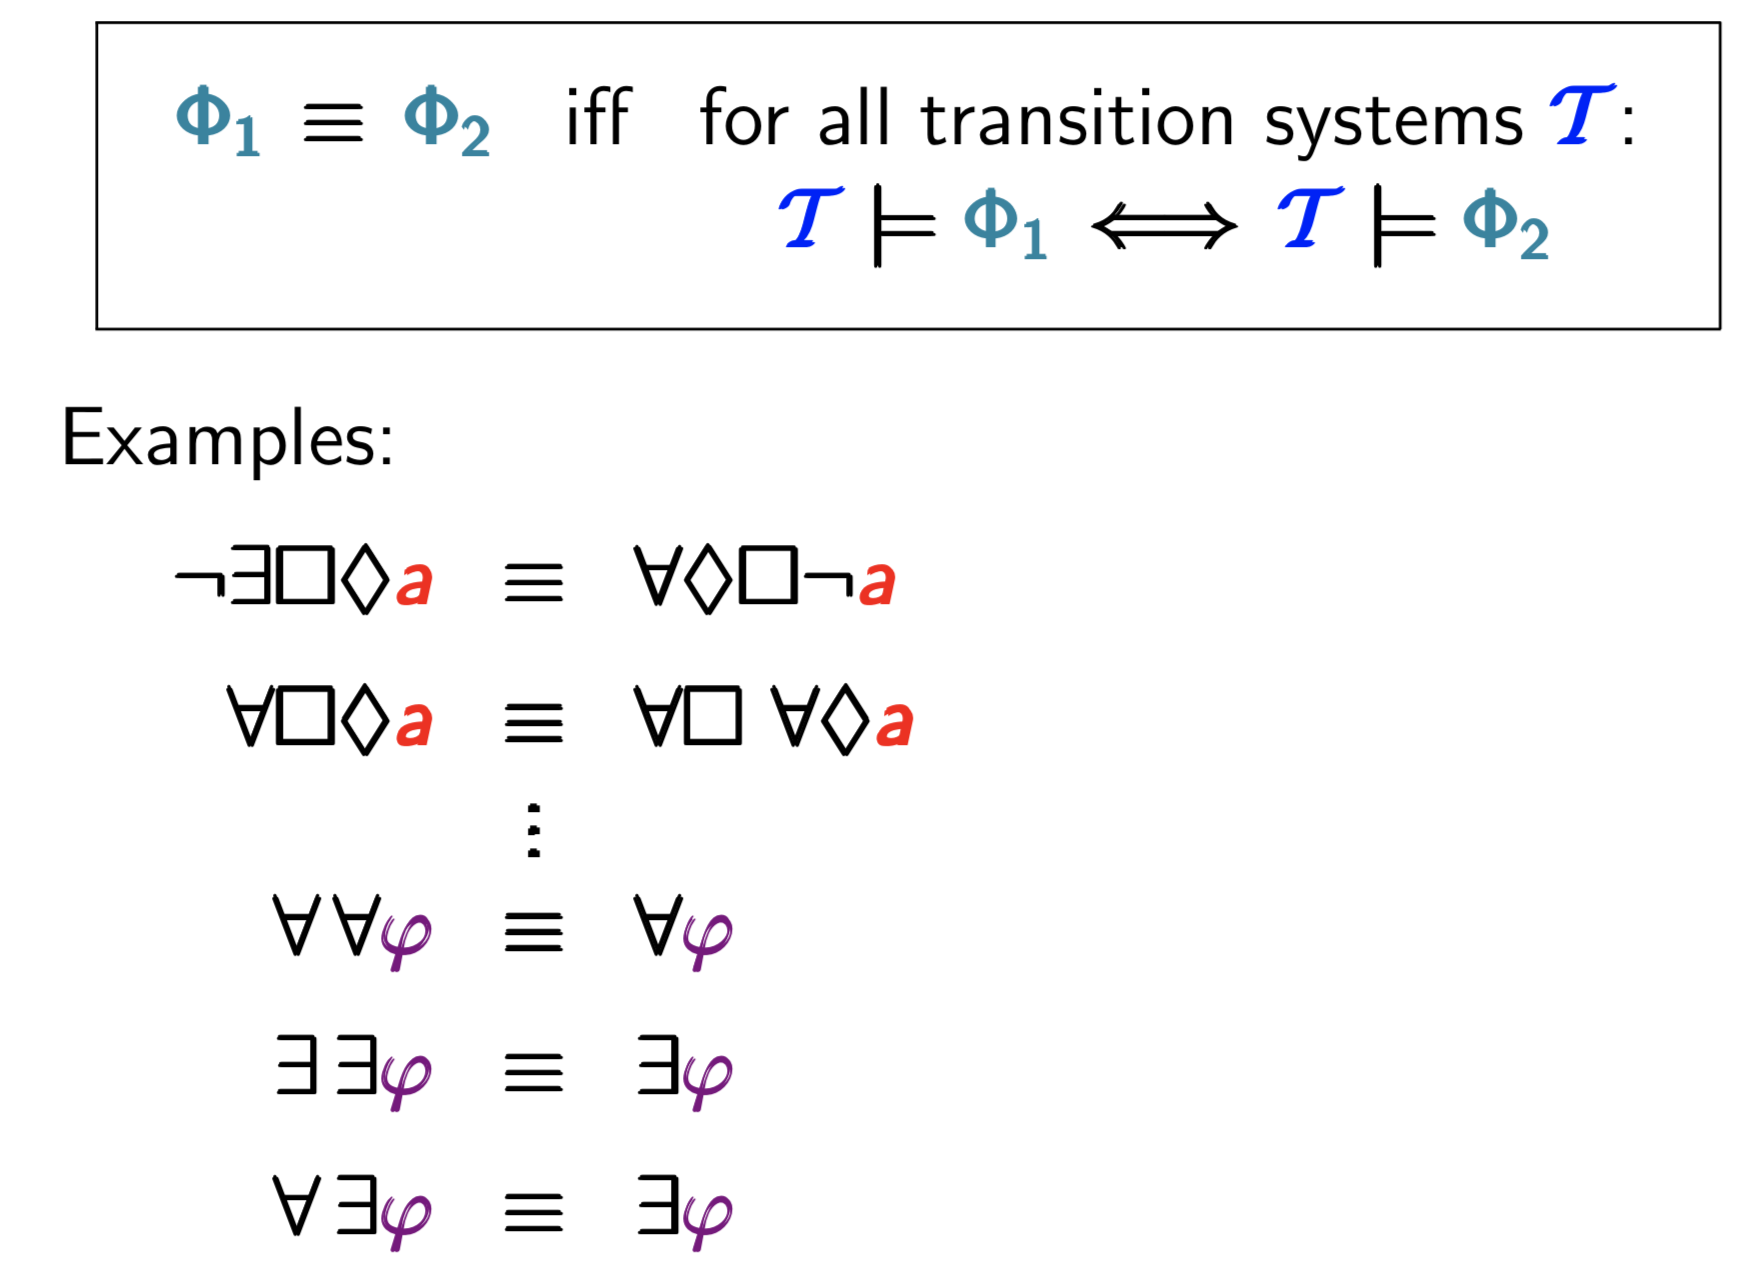
\includegraphics[scale=0.15]{*1}
	\end{figure}
	\columnbreak
	\begin{figure}[H]
		\centering
		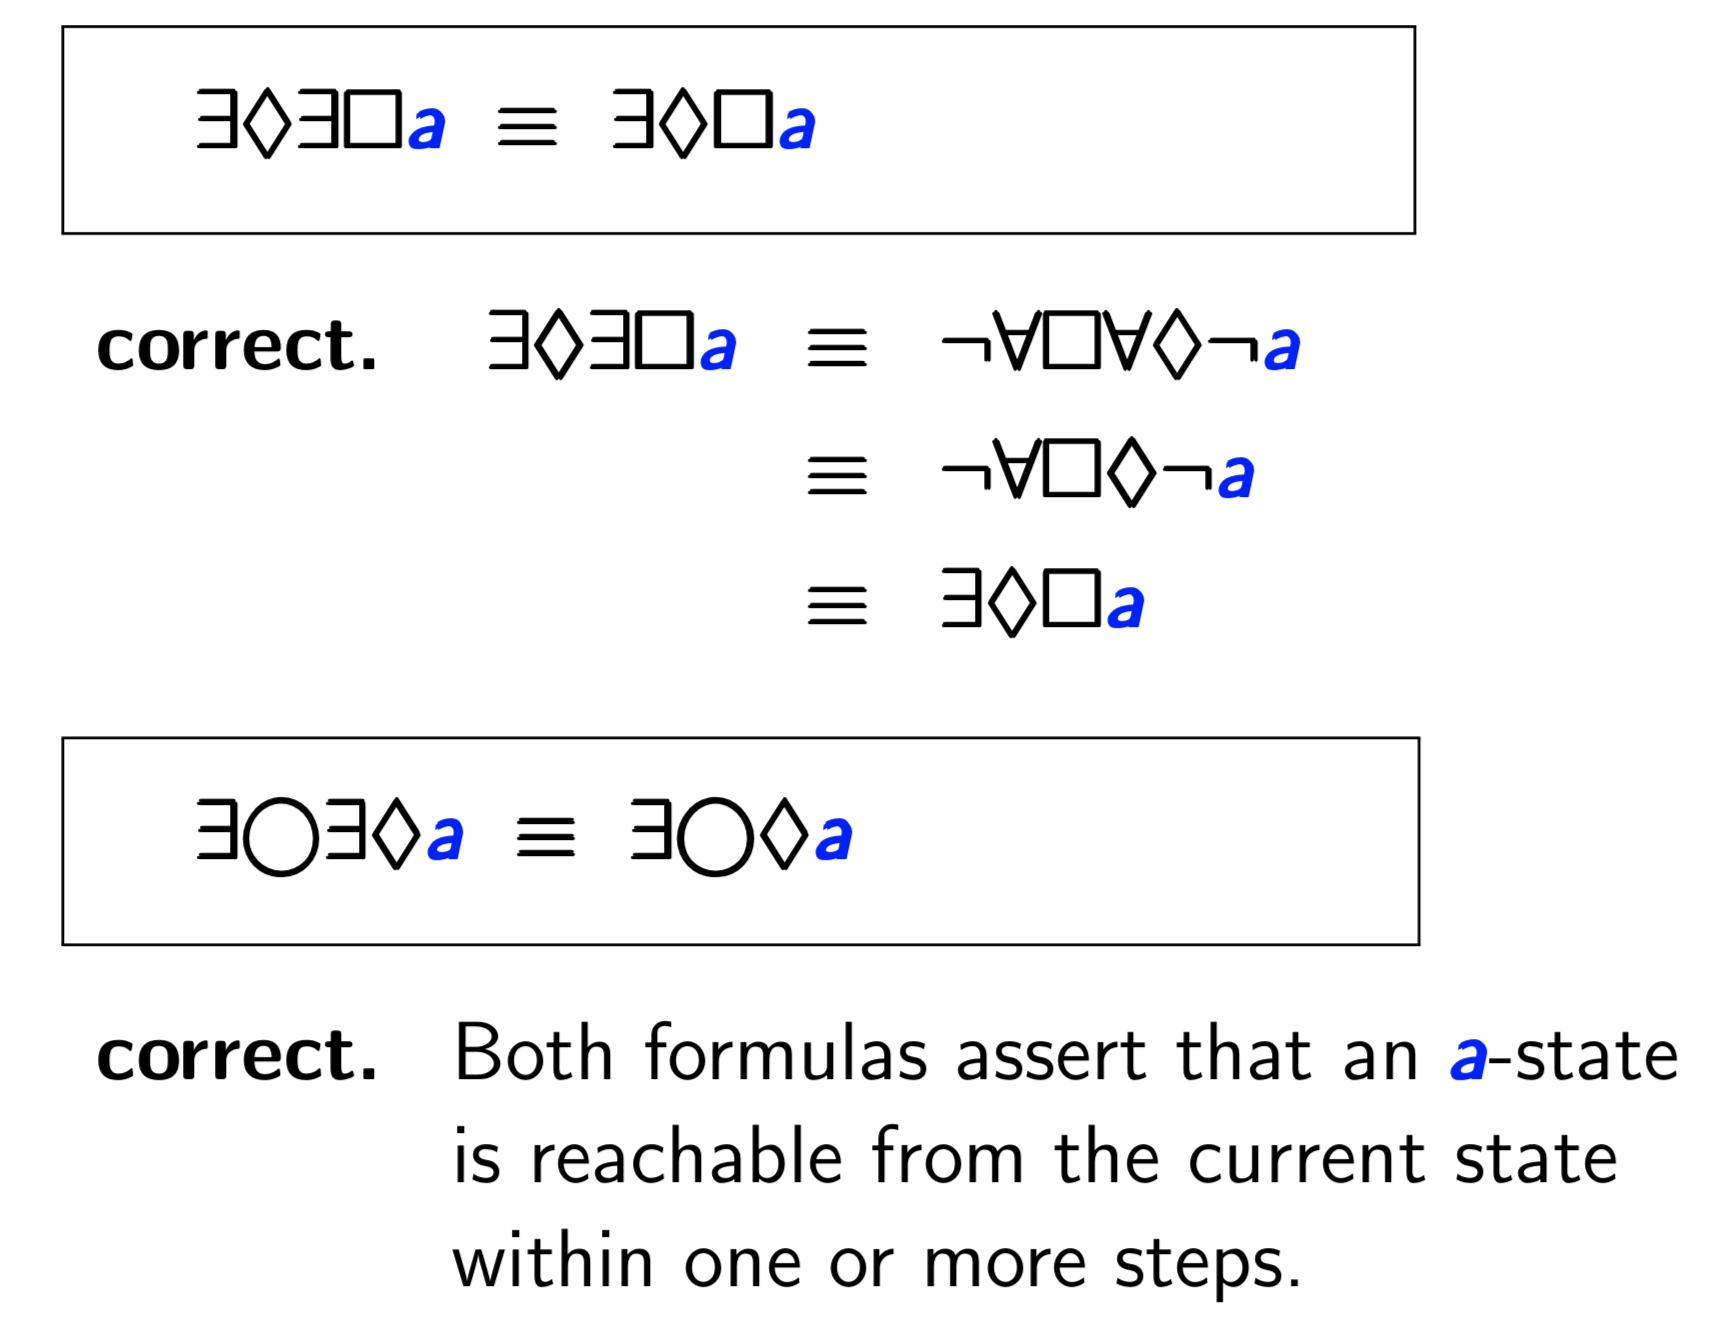
\includegraphics[scale=0.15]{*2}
	\end{figure}
\end{multicols}



\end{document}